\documentclass[12pt,a4paper,notitlepage,english]{article}
\usepackage[utf8]{inputenc}
\usepackage{amsmath}
\usepackage{amsfonts}
\usepackage{longtable}
\usepackage{amssymb}
\usepackage{graphicx}
\usepackage[a4paper, left=.6in,right=.6in,top=.8in,bottom=.8in,]{geometry}
\usepackage{tabularx,ragged2e,booktabs,caption}
\usepackage{setspace}
\setstretch{1.5}
\usepackage{tabularx, booktabs}
\usepackage{dcolumn} 
  \newcolumntype{d}[1]{D{.}{.}{#1}}    
\newcolumntype{Y}{>{\centering\arraybackslash}X}
\usepackage[T1]{fontenc}
\usepackage{babel}
\usepackage{epigraph}
\usepackage{url}
\usepackage[round,sort]{natbib}
\newcommand{\source}[1]{\caption*{\footnotesize Source: {#1}} }
\usepackage{float}
\usepackage[section]{placeins}
\usepackage{ctable}
\newcolumntype{?}{!{\vrule width 2pt}}
  \newcolumntype{d}[1]{D{.}{.}{#1}}  

\author{
  Guillaume Daudin\thanks{Université Paris-Dauphine, PSL Research University, LEDa, 75016 PARIS, FRANCE Université Paris-Dauphine, PSL Research University, IRD, LEDa, UMR 225, DIAL, 75016 PARIS, FRANCE email: guillaume.daudin@dauphine.fr}
  \and
  Elisa Tirindelli\thanks{Trinity College Dublin, email: tirindee@tcd.ie}
}
\title{How to wage a trade war? \\ Lessons from the Second Hundred Years War\thanks{The authors want to thanks Henning Hillmann and Philip Hoffman for sharing data with them. They also thanks Roger Knight, David Plouviez, Peter Solar and particpants at the IHS (London), Trinity College (Dublin) seminar in London, and at the AFSE, EHES, EHS, Réseau de Recherche pour l’innovation ad Toflit conferences}}
\date{}


\begin{document}

\maketitle


\begin{abstract}
How was Mercantilist warfare effective in its own terms, by crippling trade of defeated powers? Our paper explores the Anglo-French experience during the eighteenth century and contributes to understanding how and when this was the case. Using new French data by partner, we explore the general mechanisms relating trade and conflicts. We look into several possible candidates to explain the effectiveness of mercantilist warfare; naval supremacy, colonies loss and neutral policies. Of all the aforementioned factors, we find that the only truly efficient way to curtail the enemy commercial exchanges, was to cripple neutral trade. This strategy was the only one allowing to both decrease the enemy's trade and causing long-lasting losses.
\end{abstract}


\section{Introduction} \label{introduction}

\epigraph{Savez-vous Messieurs ce qu’est une bataille navale ? On se rencontre, on se salue, on se canonne et la mer n’en reste pas moins salée.}{Maurepas, Navy Minister of Louis  \textsc{xv}, 1718-1748}



\maketitle

Citer ?  Small and medium powers in global history: trade, conflicts and neutrality from the 18th to the 20th Centuries : edited by Jari Eloranta, Eric Golson, Peter Hedberg and Maria Cristina Moriera, London and New York, Routledge, 2019, 240 pp., &#8364;133.10 (hardback), ISBN 978-1-138-74454-7


How was mercantilist warfare \citep{Conti2017} effective in its own terms, by crippling trade of defeated powers? Our paper explores the Anglo-French experience during the eighteenth century and contributes to disentangle the effects of all the  
strategies implemented to curtail enemy's trade.
\cite{Jefferson1823} famously noticed that European nations \textit{were nations of eternal war}. Indeed, from 1700 to 1825, two years out of three experienced conflict between major European powers \citep{Roser2016}. Rivalry between Great-Britain and France was central, so much as the period between 1688 to 1815 was called the « Second Hundred Years War ». War has many causes. Yet, especially after the death of Louis XIV, it cannot be denied that mercantile rivalry was an important motivation of French wars (\cite{Wallerstein1980, Brewer2002, Crouzet2008}). Each nation was jealous of the other's commercial success. The British believed war was a good way to curtail French trade. The French partly agreed but were more wary of wars because they did not have much naval success.
Here is the long list of wars between France and Britain after the death of Louis XIV: War of the Polish Succession (1733-1738) (little naval hostilities), War of the Austrian Succession (1740,–1748, where naval hostilities started in 1744), Seven Years' War (1756–1763), War of American independence (1775–1783, where French involvement started in 1778), French Revolutionary Wars (1792–1802) and Napoleonic Wars (1803–1815).
These wars were very costly to United Kingdom \cite{Baugh1965,Neal1977,Brewer2002})
Yet, not all of these conflicts achieved their goal effectively.
Looking at figure \ref{FrBritTrade}, it is clear that French trade, despite a visible decrease in wartime, was recovering quite fast, at least until the end of the eighteenth century.
The only big exception was the period following the Continental Blockade, when the increase in trade started in the beginning of the century was brought to an end, while British trade maintained its steady growth.
Less visibly so, but as a result of some more in-depth analysis, Seven Years War also shows a similar pattern; it caused a bigger and longer-lasting effect then other similar wars.
\begin{figure}
\caption{French, British trade and Anglo-French wars}
\centering
\includegraphics[scale=.4]{"Total silver trade FR GB".png}
\source{French trade up to 1821: \cite{Daudin2020}. French trade 1822-1840: \cite{Federico2016} / \cite{Dedinger2017},

England/British trade up to 1800: \cite{Deane1969}. UK trade from 1801 to 1840: \cite{Federico2016} / \cite{Dedinger2017},

Livre tournois silver value: \cite{Dewailly1857} and \cite{Hoffman2000}; Pound sterling silver value: \cite{Clark2006} and \cite{Jastram1981}}
\label{FrBritTrade}
\end{figure}

%\begin{figure}
%\caption{Peace time trends of total French trade}
%\centering
%\includegraphics[scale=.6]{"Peace-time trends of French trade".png}
%\source{see Figure \ref{FrBritTrade} and author's computations}
%\label{FrPeaceTrade}
%\end{figure}
What were the common elements between these two wars, that made them so much more disruptive for trade? In what did they differ from the conflicts throughout the rest of the century? With this paper, we aim to uncover the strategies and the characteristics that made mercantilist war effective in its purpose.
This is important to understand the effect of wars in general, the geopolitical history of the eighteenth and nineteenth century and the globalization/deglobalization cycle from the 1490s to the 1840s.

\section{Literature} \label{literature}
There exists a vast literature focusing on the relationship between trade and war.
A first strand of this literature concentrates on the impact of trade on the occurrence of wars.
Within this strand, two major perspectives have emerged: a liberal and a realist one.
The first supports a vision of interdependence between trade and war, pointing out that trade promotes peace since it is a better method of expansion than wars (\cite{Doyle1997}, \cite{Oneal1997}, \cite{Polachek1980}).
The second opposes this view by claiming that there is no impact of trade on wars, and if any, then it will be a positive impact, as countries will be pushed to move war to maintain trade supremacy (\cite{Ripsman1996}, \cite{Levy1990}, \cite{Buzan1984})\footnote{\cite{Mcmillan1997} provides an extensive review of these two competing strands.}.
This is also dealt with, more recently, through a more quantitative approach by \cite{Martin2008}, who construct a theoretical model describing the likelihood of war and test it empirically.
They find that likelihood of war is much smaller for countries involved in bilateral trade than for those involved in multilateral.
Despite the fact that we are investigate the impact of war on trade, this literature is of interest because of the endogeneity issue.
All the aforementioned paper imply that trade may have an impact on war and therefore we may not be able to disentangle the effects of one on the other.
We argue that, in our case, this is not an issue; wars were either the consequence of exogenous events (the death of Charles VI for the war of Austrian Succession for instance) or else were the political expression of the long-lasting conflict between France and Britain.
Therefore, in our specific case, we assume that we are observing the effect of war on trade and not the reverse.\\

The second strand of the literature, on the other hand, focuses on the impact of conflicts on trade.
The works following this perspective are more homogeneous, and most authors agree to the disruptive effects on trade caused by wars.
Historians have been looking at coping strategies, e.g.  \citep{Marzagalli2006}.
Economists have been more interested in the total effect of war on trade.
\cite{Levy2004} analyse the impact of war on trade with adversary countries using seven dyads between 1870-1992, and they find that, although different across dyads, the general impact of conflict on trade is not particularly strong and mostly only temporary.
\cite{Blomberg2006} analyse more specifically the effect of all kind of conflicts, distinguishing between internal and external, and find that peace has a large and positive impact on trade.
\cite{Anderton2001} look at the effect of wars on global trade, and find that when major world power are at war significant pre and post war effects are observed, whereas impact is much smaller for conflicts between minor powers.
Finally \cite{Glick2010} try to quantify the economic impact of the two world wars and claim that conflicts had negative effects on both belligerent and neutral countries with lags up to ten years.
Altogether, the papers mentioned above do not always find coherent results, and such results were obtained from data from the last century only.
The only exception is \cite{Rahman2010} who uses British trade data from eighteen century, but concentrates manly on the impact of naval conflicts with maritime powers on trade.
The majority of scholars (apart from \cite{Levy2004}) also finds long lasting effects of war; they claim commerce took several years before restoring its prewar level.\\

The Anglo-French War in the eighteenth century was a priori destructive for trade.
Both sides used their military navies to capture  or destroy merchant shipping.
Both sides also relied on the private sector to do its part in the disruption by issuing letters of marks to authorize predation by private actors called privateers.
These actors could be either private men-of-war whose main aim was the capture of ships or merchant vessels that would have been happy to capture enemy ships if the occasion were to arose.
The importance of privateers depended on the attractiveness of alternative options \cite[p. 673]{Villiers2002,Hillmann2011}.
The impact on the French merchant fleet was especially strong during the War of American Independence \cite[table 1]{Hillmann2011}.
Merchant losses were mitigated by the widespread practice of insurance, though the loss of expected profit could no be insured. \cite[p. 160]{Ducoin1993}, \cite{Villiers2002}, \cite[p. 690-720]{Butel1973}.
In the French case, insurance rates sometimes increased so much that shipping was completely discouraged completely.
Despite the existence of insurance, merchants could not do business as usual.
Another effect of merchant shipping capture was captivity for the sailors.
They were liberated at peace time (and sometime earlier through prisoner exchange of prisoners), but mortality in British prisons was such that their capture represented a long-term loss for the French navy \cite{LeGoff1998}.
The standard response to attacks on merchant shipping was, in the eighteenth century like in the twentieth century, to organize convoys protected by military warships \cite[p. 393, 407, 448, 641]{Villiers2002}.
Despite the misgivings of merchants that saw their commercial liberty curtailed, convoys were a good solution as long as the French navy was powerful enough to defend the merchants vessels.
That was not the case during the Seven Year War or the Revolution and Napoleonic Wars.
During the Napoleonic \& Revolutionary Wars, French trade was all the more curtailed as the British became better at organizing the blockade of French ports.
There were essentially two possible types of blockades \citep{Corbett2004}; the open and the closed blockade.
The former consisted of keeping the ships at port, but ready to sail, as soon as the enemy fleet left its harbour.
This technique was much less straining for men and ships, but less efficient when it came to blockading.
On the other hand, the closed blockade consisted of keeping the rival fleet blocked in its own port, impeding it from exiting.
This was much more of an efficient technique, however, the maintenance of both ships and men at sea for such a long time was a substantial issue.
By the end of eighteenth century, the British had implemented a very efficient system of resupply, in which supply ships delivered victuals to the fleet at sea, thus allowing it not to return at port regularly for supplies.

Also, they were being very careful to provide a balanced diet against scurvy, which passed from being a major issue for sails-men, to accounting for only 2 per cent of British naval patients between 1795 and 1800.
\citep{Rodger2005}.
On top of this, British had started to coat their ships with copper, to fight the issue of barnacles, oysters and the shipworm, which were seriously hindering the speed and the security of their vessels.
This dramatically reduced the possibility of avoid the blockade and allowed British to impede unwanted trade more efficiently.
One would think that the number of ships captured declined as not many ships tried to run the blockade, but that is not confirmed by data on prizes \cite{Benjamin2009}.

Despite all these means of disruption and destruction, the effect of mercantilists wars on French trade does does not seem to have been systematic large in the long term.
\cite{Riley1986}, who concentrates on the case study of the Seven Years War, observes French trade series and he notices that there were no war lags but on the contrary pre and post war loss compensation effects.
This widely recognized fact about the effect of eighteenth century wars on French trade has led historians to research extensively the strategies of French merchants to cope with war.
=======
Also, they were being very careful to provide a balanced diet against scurvy, which passed from being a major issue for sails-men, to accounting for only 2 per cent of British naval patients between 1795 and 1800 \citep{Rodger2005}.
On top of this, British had started to coat their ships with copper, to fight the issue of barnacles, oysters and the shipworm, which were seriously hindering the speed and the security of their vessels.
This dramatically reduced the possibility of avoid the blockade and allowed British to impede unwanted trade more efficiently.
One would think that the number of ships captured declined as not many ships tried to run the blockade, but that is not confirmed by data on prizes \citep{Benjamin2009}.

All these means of disruption and destruction forced French trade to adapt (e.g. by increasing land trade, see Figure  \ref{Share_by_sea} ).
Still, the effect of mercantilists wars on French trade does not seem to have been systematically large in the long term.
\cite{Riley1986}, who concentrates on the case study of the Seven Years War, observes French trade series and notices that there were no war lags but on the contrary pre and post war loss compensation effects.
This widely recognized fact about the effect of eighteenth century wars on French trade has led historians to research extensively the strategies of European merchants to cope with war..
>>>>>>> origin/master
Neutral carriers were somewhat protected from British predation on the sea.
When necessary, French merchants could even hide their cargo ownership behind a neutral partner.
Or they could move to neutral countries and operate from there \citep{Marzagalli2016}.
Historians have even reflected that war periods might have been necessary to the functioning of the \textit{Exclusif Colonial}, i.e. the theoretical monopoly of French merchants on French colonial trade \citep{Lespagnol1997, Morineau1997, Marzagalli2016}.
The argument rests on the large peace time trade imbalances between France and its Northern European clients for colonial goods that could have been balanced by large service income of Northern European merchants during war time as they, as neutrals, provided shipping and various trade services to the French empire.
The quality of the available balance of payment data is not good enough to test that hypothesis.
Along these lines, \cite{Juhasz2018} finds that regions of the French Empire which were protected from trade with the British during the Continental Blockade increased capacity in mechanized cotton spinning to a larger extent than regions which remained more exposed to trade.\\


\begin{figure}
	\caption{Share of French trade conducted by sea}
	\centering
	\includegraphics[scale=.4]{"Share_by_sea".png}
	\source{TOFLIT and 1792 data on the share of sea trade per country in AN F/12/1834 B}
	\label{Share_by_sea}
\end{figure}


The aim of this paper is to extend \cite{Riley1986}’s work by analysing the available French data in the eighteenth century.
So far the literature has mainly analysed the impact on trade of twentieth century wars and generalized the results.
We believe that the effect of wars in twentieth century is different from that of other wars throughout history, and related data offer only a partial point of view.
Thus, we are convinced that analysing data older than twentieth century is crucial to understand the general mechanisms relating trade and conflicts.
We construct a loss measure for trade throughout the century and we find that indeed the main losses took place during Seven Years War and Revolutionary \& Napoleonic Wars.
We explore several possible causes and we find that the common factor in case of major disruption was the policy adopted towards neutral countries.
This leads us to think that wars were not a big source of disruption for trade, as long as neutral countries were allowed to trade relatively freely and take over the trade from belligerent countries.
It was only during the Seven Years Wars and the Napoleonic \& Revolutionary Wars, when commerce with neutral countries was also restricted, that French trade experienced a massive decline \citep{Findlay2009}.
This decline was long-term and put an end to the competition for trade supremacy in Europe, which was ultimately won by the United Kingdom, by the end of the century.
This avails the hypothesis of the role of neutral countries in modern trade and its importance for its success.


\cite{Rahman2010}  shows that fighting a naval power with a large navy is bad for trade. The close examination of the mercantilist rivalry between Britain and France clarifies the channels through which a naval power can do long-term damage one's trade.



\section{Dataset} \label{dataset}
\subsection{Sources of the data} \label{sources_of_data}
We use data from the TOFLIT18 project (see http://toflit18.medialab.sciences-po.fr/\#/home). They come from the archives of the French \textit{Bureau de la Balance du Commerce} and, subsequentely, the \textit{Bureau des archives du commerce}.
This institution was created in 1713, after the Treaty of Utrecht, which followed the Spanish Succession War.
While discussing a trade treaty with the British, the French negotiators were positively impressed by the detailed knowledge shown on actual trade flows by their counterparts , and they convinced the government of the necessity of creating an institution that would keep track of exports and imports from and to France \citep{Charles2011}\footnote{\cite{Charles2011}, in their paper, provide the complete history of the \textit{Bureau}.}.
Starting with the year 1716, local \textit{bureaux des fermes} sent their trade records to the \textit{Bureau} in Paris.
The \textit{Bureau} would then compute aggregate yearly figures for each \textit{direction} (port) and then send them back to the local Chamber of Commerce, so that they could add the values up to 1780.
A mix of local and central source survive from this process. Unfortunately these "local sources" mostly did not survive; what we have left are parts of the centralised records.
From 1781 to 1791, the work methods of the Bureau changed and a number of years of trade have left little record (1783-1786, 1790-1791).
In 1792, through a decree of the National Assembly, the \textit{Bureau de la Balance du commerce} was abolished and replaced by the \textit{Bureau des archives du commerce}. We have some data on 1792 trade, but trade collection started again in earnest in 1797, so that we are missing information on 1793-1796.\\
The data that have survived is contained in different kinds of documents.
The two most exhaustive ones contain trade by product and per partner. They were the \textit{Objet Général}, between 1754 and 1780, 1782 and 1788. Some years are missing, especially in the the period between 1761 and 1767, and the \textit{Résumé}, between 1787 and 1789 and between 1797 and 1821.
The \textit{Objet Général }includes the value of the flows and, from 1771, it includes also quantities and / or unit prices.
The \textit{Résumé} does not include quantities, only values. The classification of goods it uses is less precise than the one from the \textit{Objet Général}.
Local trade data are available from 1716 to 1780 and in 1789. These sometimes allow partial reconstruction of total French trade (see \ref{composition}).
Very importantly for the first part of the analysis, a \textit{Tableau Général} exists in the French archives that provides French bilateral trade (though it is not broken down by product) (\cite{Romano1957}). \\
Our sources provide the value of trade in the current French currency. This is the \textit{livre tournois} up to 1795 and the \textit{franc} afterward. The value of the \textit{livre} was fluctuating in the early eighteenth century. In 1726, its value was fixed at a value of 4.505 grams of fine silver \citep{Dewailly1857}. Because of the monetary crisis during the revolution, we use data extracted from published appreciation tables to fix the value of the \textit{livre} at 2.9 grams of silver in 1792 (\cite{Hoffman2000}) . The French franc contained 4.5 grams of fine silver. We convert most trade flows in fine silver ; obviously, this does not solve the inflation issue, but inflation in terms of silver was relatively limited during that period.

\subsection{Trade partners} \label{figures}
Trade partners are not consistently designed in the original data. 
For example, In the \textit{Tableau Général} (from 1716 to 1782), the number of partners varies between 14 and 23 and between  16 and 26 in the \textit{Résumé} (from 1787 to 1821).
Often, partners are not single countries but rather groups of countries.
Many destinations get broken down into smaller destinations in later periods or even disappear to be replaced by other smaller entities.
To bypass this problem we have created a classification of countries, which is consistent for the whole period (such that we have nearly one observation for each group for each year).
This classification identifies only twelve groups: \textit{Allemagne}, \textit{Angleterre}, \textit{Espagne}, \textit{Flandre et autres États de l'Empereur}, \textit{Hollande}, \textit{Portugal}, \textit{Suisse}, \textit{Levant}, \textit{Italie},  \textit{États-Unis}, \textit{Outre-mers} and \textit{Nord}. Many are self-explanatory, though it should be underlined that trade with \textit{Angleterre}, \textit{Portugal} and \textit{Espagne} includes trade with all their controlled territories. \\
\textit{Outre-mers} regroups all intercontinental French trade (mainly with French colonies) except for North Africa and the Ottoman Empire that are included (along with Greece) in  \textit{Levant}.\\
\textit{Nord} designates trade north of the Low Countries.
This region comprises Sweden, Denmark, Hanseatic ports (mainly Hamburg, Bremen, Lubeck and Danzig), Prussia and Russia\footnote{Trade with Denmark is identified separately from 1733, trade with Sweden from 1734 and trade with Russia from 1744.
We always account for them together under \textit{Nord}} \citep{Charles2018}.\\
\textit{Italie} was used as a geographical expression.
The main French trade partners there were the Kingdom of Piedmont and Sardinia and Genoa.
Still, minor flows were also directed to Milan, Naples, Venice, Tuscany, Papal States...\\
\textit{Flandre et autres États de l'Empereur}  (\textit{Empereur} for short) is mainly modern Belgium before the Revolutionary and Napoleonic Wars and mainly Austria after it. At that point, modern Belgium is annexed by \textit{Hollande}. \\
\textit{Allemagne} encompasses mainly Western Germany, including Alsace, Lorraine during the \textit{Ancien Régime}. \\
We have not attempted to take into account the extensive territorial re-arrangements during the Revolutionary and Napoleonic Wars.
The extension of France in the Low Countries, Germany and Italy changed the actual extent of the \textit{Allemagne} and \textit{Italie} partner.


\section{Historical summary} \label{historical_summary}
As mentioned above, the eighteenth century was a period of "eternal war".
In fact, between 1716 and 1820, two out of three years experienced a conflict.
In this section we provide a brief overview of the main wars that took place in Europe in the period of analysis and we explain how we classified the belligerent status (compared to France) of the country groupings we use. We always consider \textit{Outre-mers} as ally and \textit{Levant} as neutral\\
In 1733, the king of Poland August \textsc{ii}, died heirless and his succession soon became a conflict at European level.
France, Prussia and Spain were trying to limit the desire of expansion of the Habsburg monarchy in Poland. Britain stayed neutal and the war concluded in 1738, with the recognition of August \textsc{iii} as king of Poland, as the Habsburg had wished and France gainining .
In the country classification we used, the ally countries were \textit{Espagne}  and the foe was \textit{Empereur} and and \textit{Allemagne} (as Lorraine and West Germany were at that point mostly controlled by the Habsburg).
It was a land conflict, as opposed to the naval conflicts that followed. \\
No longer than two years later, a very similar event occurred as a consequence of the death of Charles \textsc{iv}.
The Habsburg emperor had not died heirless, however his only heir was a woman; Maria Theresa of Austria.
France, Prussia and the Electorate of Bavaria used the pretext that she was ineligible to succeed to her father, to challenge, once again, the Habsburg power.
Maria Theresa was supported by the Kingdom of Great Britain and the Dutch Republic as well as the Kingdom of Sardinia and the Electorate of Saxony.
This conflict, which was born as a succession issue, soon extended to the New World and became a competition between the French and the British for the control of American colonies.
It ended in 1748 with the Treaty of Aix la Chapelle, where France gave back most the territories it had conquered during the war.
Ally country in this case was \textit{Espagne} and foes were \textit{Angleterre} and \textit{Empereur}. \\
Roughly until the end of the Austrian Succession war, a sort of geopolitical and economic equilibrium between France and British colonies on the North American mainland had prevailed. That was broken as a consequence of an uneven population growth \citep{Findlay2009}.
This set the stage to the following war; the Seven Years War, or French and Indian War, which, as the name suggests, was a world-wide conflict.
As opposed to the previous wars, this was a decisive triumph of Britain over France, which was forced to give up Canada, Cape Breton Island and Grenada, recognized the Mississippi River as the Eastern boundary of its possessions in North American, then ceded those possession to Spain.
France also lost enough influence in its colonies to lead to the end of French colonial ambition in India and, subsequently, to the dissolution of the first Compagnies des Indes \citep{Riley1986}.
French allies in this war were \textit{Allemagne}\footnote{As mentioned in section \ref{dataset}, \textit{Allemagne} was mainly Alsace, Lorraine and Western Germany, which were allied to France.
Our assumption is that "Prussia" is sea trade through the Baltic, i.e. a minor portion of \textit{North}, which, however we code as neutral, since it was dominated by Hamburg - despite the fact that Russia and Sweden were allied to France for most of the war.}, \textit{Empereur}, and \textit{Espagne} for 1762.
Foes were \textit{Angleterre}, and \textit{Portugal}. \\
At the end of the Seven Years War, with the victory of Britain and the subsequent departure of the French, the American colonies, no longer feeling the threat of the French presence on the continent, soon started demanding independence from Great Britain\footnote{The French chief minister, the duc the Choiseul, made a prediction to the effect that with no French presence on the continent to threaten them any longer, the American colonies would soon demand independence from Great Britain \citep{Findlay2009}.
This prediction, as it turned out, was prescient.}.
In 1775 they rebelled against British control over their trade and in 1776 they declared independence.
France, still feeling the humiliation subsequent to the Seven Year War, in 1778 entered the fray on the colonies' side, soon followed by Spain.
Spanish and French \footnote{France had been investing in its Navy following the preceding defeat \citep{Findlay2009}.} fleet together outnumbered the British Navy and were able to force Britain to surrender and end the war with the Treaty of Versaille in 1783.
In this setting, ally were there \textit{Espagne}, \textit{Etats-Unis}, and \textit{Hollande} from 1780; foe was only \textit{Angleterre}. \\
At the end of the war, despite the victory obtained, French finances were suffering to the extent that Calonne, the finance minister at the time, was forced to the summoning of the Estates-Generales in 1789, which then led to the start of the French Revolution.
This event was followed by a larger conflagration with respect to previous mercanilist wars, into which an ideological dimension had been injected \citep{ORourke2006}.
In 1792 France declared war on Austria and Prussia, and the following year to Great Britain.
The subsequent conflict lasted for nearly thirty years, with only two brief interruption between 1802 and 1803 (Peace of Amiens) and between 1814 and 1815.
Almost immediately, France banned the import of all British goods; Britain responded by blockading French coasts and impeding French ships to exit the port.
From the very beginning, this created a big problem for neutral countries, which wished to continue trade with both belligerent actors.
As a consequence, a second League of Armed Neutrality was created, in which Russia, Prussia, Denmark and Sweden took part.
This alliance was not long-lasting, as Britain responded with a ban on trade with the league, and bombed Copenhagen, thus ending this agreement.
This conflict ultimately ended with Napoleon's disastrous invasion of Russia in 1812, which was followed by the invasion of France in 1814 and a subsequent peace treaty signed in Ghent.
The two main players of this conflict were, of course, Britain and France.
However, because of the victories and defeats of one and the other, sides of other countries changed continuously and it was harder to code in our country classification. Table \ref{war_peace} reports our choices of the position of all countries in all wars throughout the century. 
\textit{Allemagne} was mainly aligned with Austria till 1800: so it was a foe between 1792 and 1800, neutral between Campo Formio became an ally in 1805 (till 1813), and then became again a foe after the battle of Leipzig to France.
\textit{Angleterre} was an enemy all throughout.
\textit{Espagne} fought France for the period 1793 and 1794, she became then an ally until 1807 (with the exception of 1795, in which she was neutral), and then again an enemy from 1808 onwards.
\textit{Empereur} is Austria, whose position was easy to adjudicate. It was a foe until Campo Formio (June 1801), neutral till the Third Coalition (1805), then a foe in 1805, to become neutral again in 1806 until 1808.
Lastly, after one more year of neutrality in 1809, she became an ally starting from 1810, and declared war again in 1813.
\textit{Etats Unis} was always neutral throughout the war, except for the un-declared war between 1798 and 1800.
\textit{Hollande} fought France till 1794 and was then aligned to it till late 1813, when William-Frederik of Orange-Nassau took power.
\textit{Italy} was briefly a foe until 1796, then neutral until 1813, and then again a foe starting 1814.
\textit{Levant} stayed out of the war, except when the French invaded Egypt from 1798 to 1801.
Concerning \textit{Nord}, Sweden and Russia were alternatively neutral, foes or allies. Denmark was an ally. Yet, as the biggest share of trade was represented by Hamburg, whenever the component of \textit{Nord} were not on the same side in a war, we code them all in the position of Hamburg. \textit{Nord} was mainly neutral, except when it was occupied and then annexed by France from 1808 to 1813.\footnote{Obviously, we cannot proceed this way for the computation of naval supremacy, see \textit{infra}.}
\textit{Outre-mers} mainly includes French colonies and we treat it as an ally throughout.
\textit{Portugal} was neutral until 1798 and then became a foe in 1802.
It was again neutral for a short period between 1803 to 1806 and then became a foe starting from 1807.
Finally, \textit{Suisse} was neutral until 1797 and then an ally until 1813, and then neutral again in 1814. \\



\begin{table}
\centering
\caption{Summary of war status for trade partners, 1792-1815}\label{war_peace}
\begin{tabular}{?c|c|c|c?}
\specialrule{.15em}{.1em}{.1em}
\textbf{Country}    & \textbf{Foe}       & \textbf{Neutral}   & \textbf{Ally}   \\ \specialrule{.15em}{.1em}{.1em}
Allemagne  & 1792-1800 & 1801-1804 & 1805-1813   \\
           & 1814-1815 &           &             \\
Angleterre & 1793-1815 & 1792      &             \\
		   &           &           &               \\
Espagne    & 1793-1794 & 1792      & 1796-1807   \\
           & 1808-1815 & 1795      &  		  \\
Empereur   & 1792-1800 & 1801-1804 & 1810-1812    \\
           & 1805      & 1806-1808 &           \\
           & 1809      &           &           \\
           & 1813-1815 &           &          \\
États-Unis & 1798-1800      & 1792-1797 & \\
			&&1801-1815& \\ 
Hollande   & 1793-1794 & 1792           & 1795-1813 \\
           & 1814-1815 &           &           \\ 
Italie    & 1792-1796 &  & 1797-1813 \\
          & 1814-1815 &           &   \\ 
Levant    &  1798-1801         & 1792-1797 &  \\ 
			&&1802-1815&  \\
Nord      &  & 1792-1807 & 1808-1813  \\   
		 & & 1814-1815 & \\
Outre-mers &           &           & 1792-1815   \\ 
Portugal & 1793-1797& 1792 &       \\       
          &1799-1800  &1798 &   \\ 
          &1807-1815 &1801-1806 & \\
Suisse    &           & 1792-1797 & 1798-1813 \\
		  &             & 1814-1815 & \\


                    
\specialrule{.15em}{.1em}{.1em}  
\end{tabular}
\end{table} 




Figure \ref{Number_of_protagonists} sums up the data by showing the number of French allies, foes and neutral for each war and year of interest. \\
\begin{center}
\begin{figure}[H]
\caption{Number of protagonists}
\label{Number_of_protagonists}
\centering
\includegraphics[scale=1]{"Number of protagonists".pdf}
\end{figure}
\end{center}


\section{Empirical Analysis} \label{analysis}
The aim of this study is to uncover the effects of the long-lasting war status that marked the eighteenth century and to identify the drivers of the massive loss in trade associated to some of these conflicts. \\ 


%We construct a loss measure for trade throughout the century and we find that indeed the main losses took place during Seven Years War and Revolutionary Wars.

\subsection{Explained variable}
%LOSS FUNCTION
We start by defining a loss function of the effects of wars.
We construct it as the percent loss, compared to past peace time trend.
\begin{equation*}
Loss = \frac{Expected \> value \> based \> on \>past \> peace \>trend - Observed \> value}{Expected \> value \> based \> on \>past \> peace \>trend}
\end{equation*}
Figure \ref{annual_loss_function} shows the annual loss function for the period of interest. Figure \ref{mean_loss_function} shows the mean loss function by peace or war period.
The black dotted line shows observed trade versus trade predicted based on all preceding peace period, whereas the red solid line shows the comparison with the prediction based on the single preceding peace period only.
\footnote{We exclude 1792 from the computation of peace time trends when we take into account only the preceeding peace period. Its value, in a era of inflation, is doubtfull and there are very limited peace years with data available from 1784 to 1792 : only 4 (including 1792). Including it increases the past peace time trend for the pre-1815 period from 1.4 p.c. to 2.9 p.c. Including it does not change much when computing the peace trend based on all past peace periods : it stays at 2.65 pc)}
This graph shows that the most successful wars from the point of view of Britain, trying to disrupt French trade, were the Revolutionary \& Napoleonic War and the Seven Years War.
The loss function is higher during these conflicts (more than 40\% and 60\%) than during the Austrian Succession War and the American Revolutionary War (respectively 20\% and 30\%).
Furthermore, the loss function is positive also after the war, whereas it is negative after the Austrian Succession War and the American Revolutionary War. The disruption of French trade lasted through peacetime for these two wars. 
Therefore, at a first glance, these two conflicts were more harmful to trade than others.
Looking at figure \ref{mean_loss_function} makes this point stronger.
We observe, in fact, that post-Seven Years War loss (during peace) is roughly comparable to the war-time loss during the American Revolutionary War altogether.
It is undoubtedly hard to disentangle the effect of the American Revolutionary War itself and the lags from the preceding war, however, whatever the distribution of weights between these two events, it is undeniable that the consequences of the Seven Year War were quite significant.
The same holds for the Revolutionary \& Napoleonic Wars, which have been long identified in the literature as a major cause in French trade disruption at the end of the nineteenth century \citep{ORourke2006}. \\
In an analogous way we have computed the loss function for UK trade (figures \ref{GBannual_loss_function} and \ref{GBmean_loss_function}). What we observe here is that, first of all, losses are much less significant than for France for the overall period. In particular, the loss function is negative 1756 and 1778 and after 1781, at least while using all past period to predict the trend. This suggests that, although the British may not have been successful in curtailing French trade, they were nonetheless profiting from some conflicts for their own commerce. 

\begin{center}
\begin{figure}[H]
\caption{Annual Loss Function}
\label{annual_loss_function}
\centering
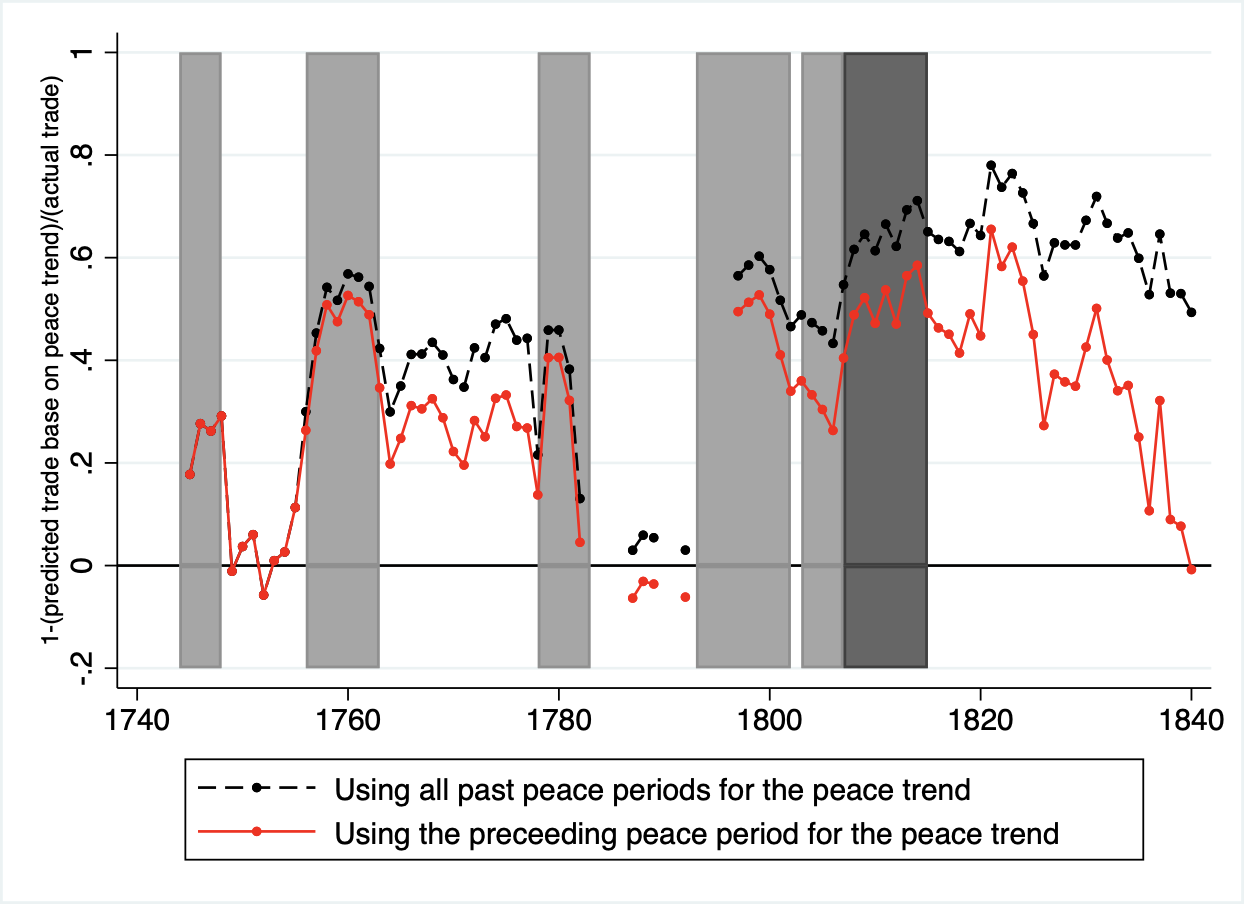
\includegraphics[scale=.425]{Annual_loss_function.png}
\caption{Mean Loss Function}
\label{mean_loss_function}
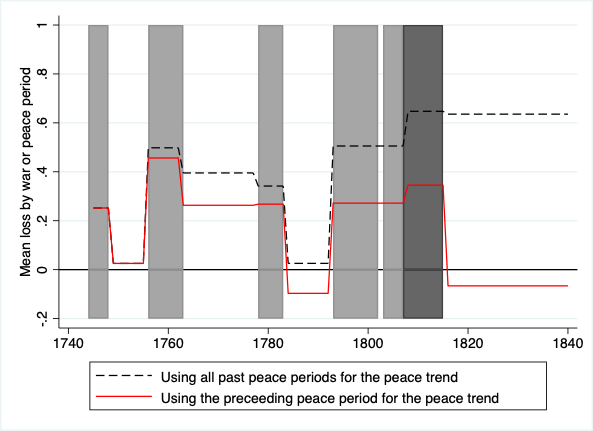
\includegraphics[scale=.4]{Mean_loss_function.png}
\end{figure}
\end{center}

\begin{center}
\begin{figure}[H]
\caption{GB Annual Loss Function}
\label{GBannual_loss_function}
\centering
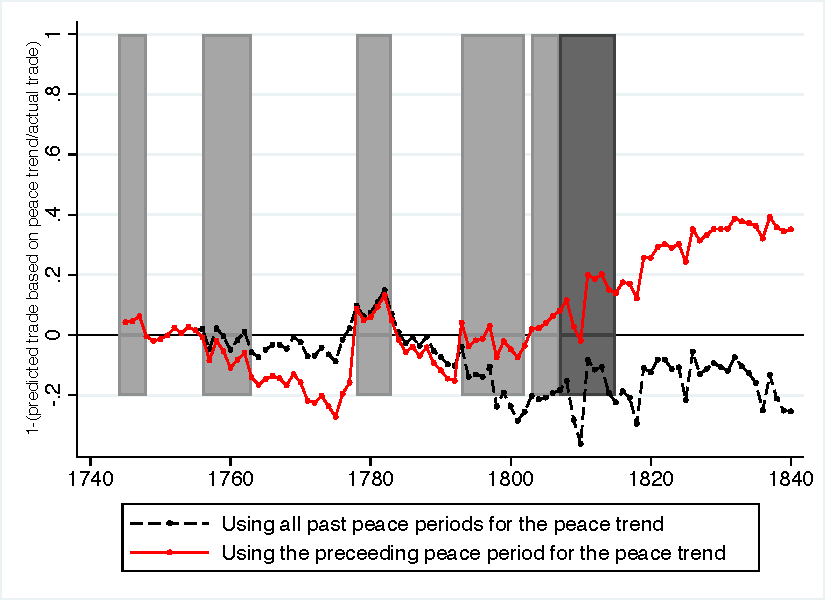
\includegraphics[scale=0.9]{GBAnnual_loss_function.pdf}
\caption{GB Mean Loss Function}
\label{GBmean_loss_function}
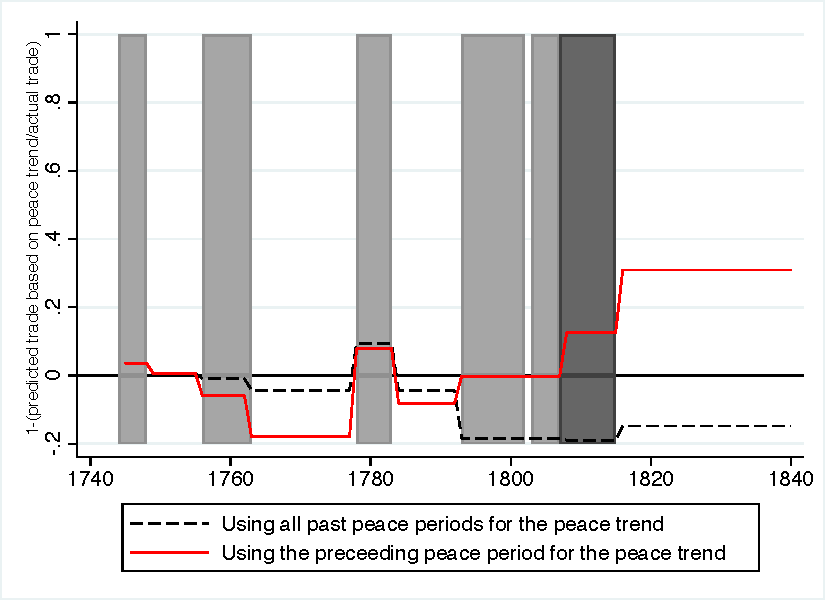
\includegraphics[scale=0.9]{GBMean_loss_function.pdf}
\end{figure}
\end{center}

\subsection{Can we do a cost-benefit analysis?}
In a cost-benefit analysis of the efficiency of the British war on French trade, the reduction of French trade would be a good place to start to look at the benefits. Though, the cost for the French economy is not the reduction in trade per se. It is more precisely the loss of economic activity entailed by the reduction in trade. What were the decrease in wages and profits, both for French actors of trade and French producer? This is a tricky question. Daudin (\cite[p. 408]{Daudin2005}) evaluate the income of French actor at 38.5\% of the value of intercontinental trade and 27.5-35\% of the total value of trade. Intercontinental trade was more affected by the British war on French trade, so maybe we should favor the higher estimate. On the other hand, at least part of the workers, entrepreneurs and capital could find alternative use and did not stand completely idle after the reduction of trade. \cite[p. 421]{Daudin2005} evaluate the loss 40\% of the value of the production. If we take these numbers seriously, it means a 100 livres tournois declined in the value of French trade forced workers, entrepreneurs, capitalists earning 35 livres tournois to find another employment for their labor and their capital. This other occupation only yielded an income of 21 livres tournois, and hence to a loss of 14 livres tournois for French GDP. This number is highly uncertain. \cite{Daudin2005} argues we should take into account the dynamic effect of this income loss through lost savings and investments.

We can include in French losses the French expenditures on its military Navy, as one of its important aim was to protect trade.  The French Navy budget data stops in 1782 \cite{Acerra1997, Villiers1997,Petitfils2015}). The French Navy budget was always smaller than the British one.

We should add to French loss the destruction or capture of French ships. This is tentatively possible thanks to information French prizes captured both by the British Navy and British privateers, discussed in section \ref{section:DestructionofFrenchshipping}\footnote{From 1793 onward, we use the data on the value of Navy Prizes from \cite{Benjamin2009}, based on \cite{Hill1998}. Before that period (and from 1793 for privateers) the data come from \cite{Starkey1990,Hillmann2011}. Before 1793, we assume the same median value and share of French prize for the Navy Prizes that what is available for privateers }. 

Finally, how much did Britain pay to reduce French GDP? Again, that is probably not possible to compute. A good place to start, though, is the budget of the British Navy. \cite[pp. 570-587]{mitchell1988} provides the net expenditures up to 1801 (1800 is incomplete)) and the gross ones from 1802.

Figure \ref{Expenditures} presents these data. Except for the War of the American Independance, the French Navy budget always was smaller than the British one. The total value of prizes was rather small, apart during the early Seven Years War.

\begin{center}
	\begin{figure}[H]
		\caption{British Navy budget and French trade losses}
		\label{Expenditures}
		\centering
		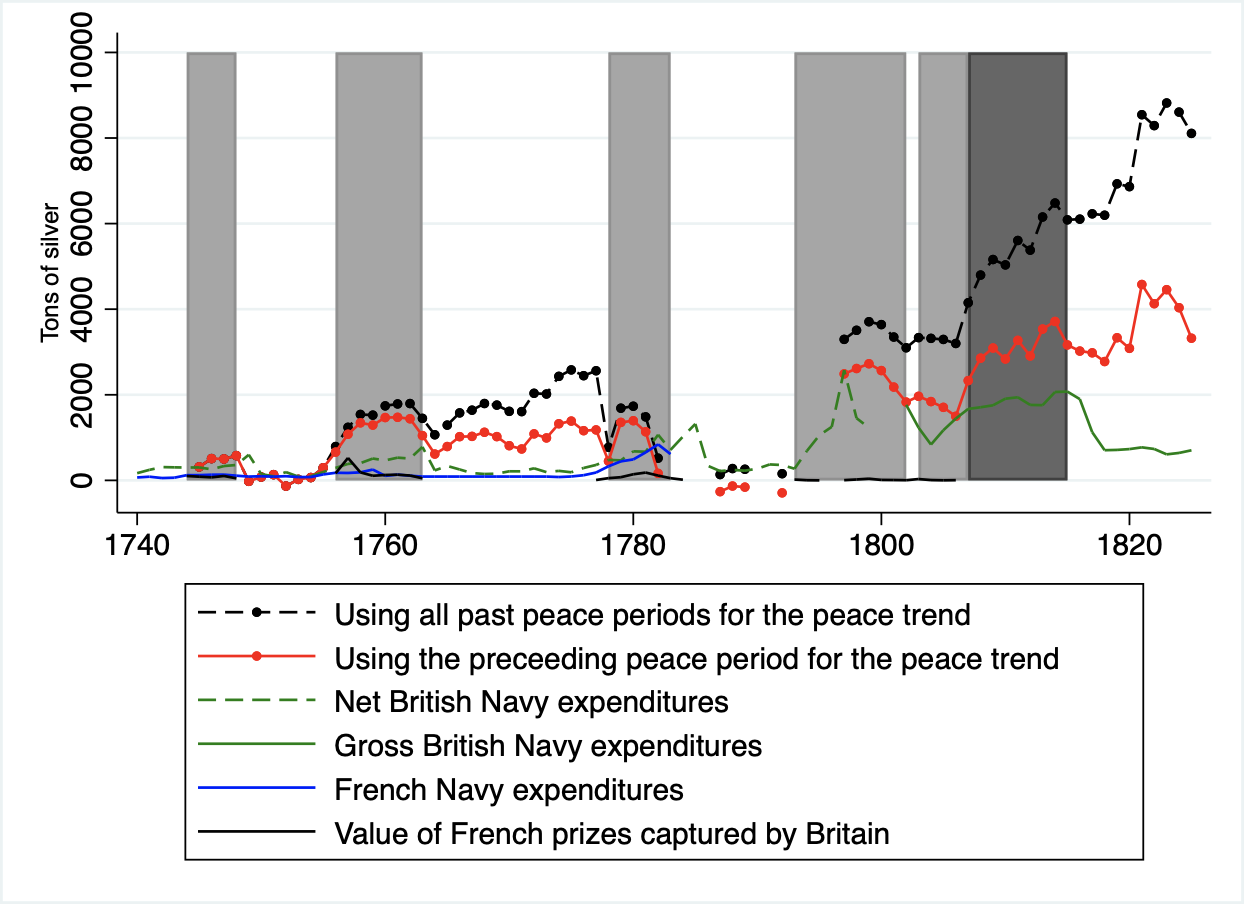
\includegraphics[scale=0.5]{Expenditures_Annual_Loss.png}
		\source{See text and \cite[pp. 570-587]{mitchell1988}}
	\end{figure}
\end{center}


Figure \ref{Ratio_BR_Expenditures} compares the cumulated British expenditures and French losses. At value less than one means that the war on trade is costing more ressources to the British than to the French (neglecting the value of French prizes). they are denying ressources from the French.  The "high" hypothesis is the most favorable to the policy, as it assumes that French labor and French capital invested in trade just become unemployed when trade is reduced: hence French income losses are 35\% of French trade losses. The "low" hypothesis is probably more reasonable and assume that French labor and capital find alternative, less remunerating, employment: hence French income losses are 14\% of French trade losses.
Prizes are pretty important in the cost/benefit analysis during the Seven Years War, in part because of the success of the British predation of French trade before the official declaration of war, but they loose their importance in the latter part of the period.


\begin{center}
	\begin{figure}[H]
		\caption{Ratio between French trade losses and the British Navy budget, high and low hypothesis}
		\label{Ratio_BR_Expenditures}
		\centering
		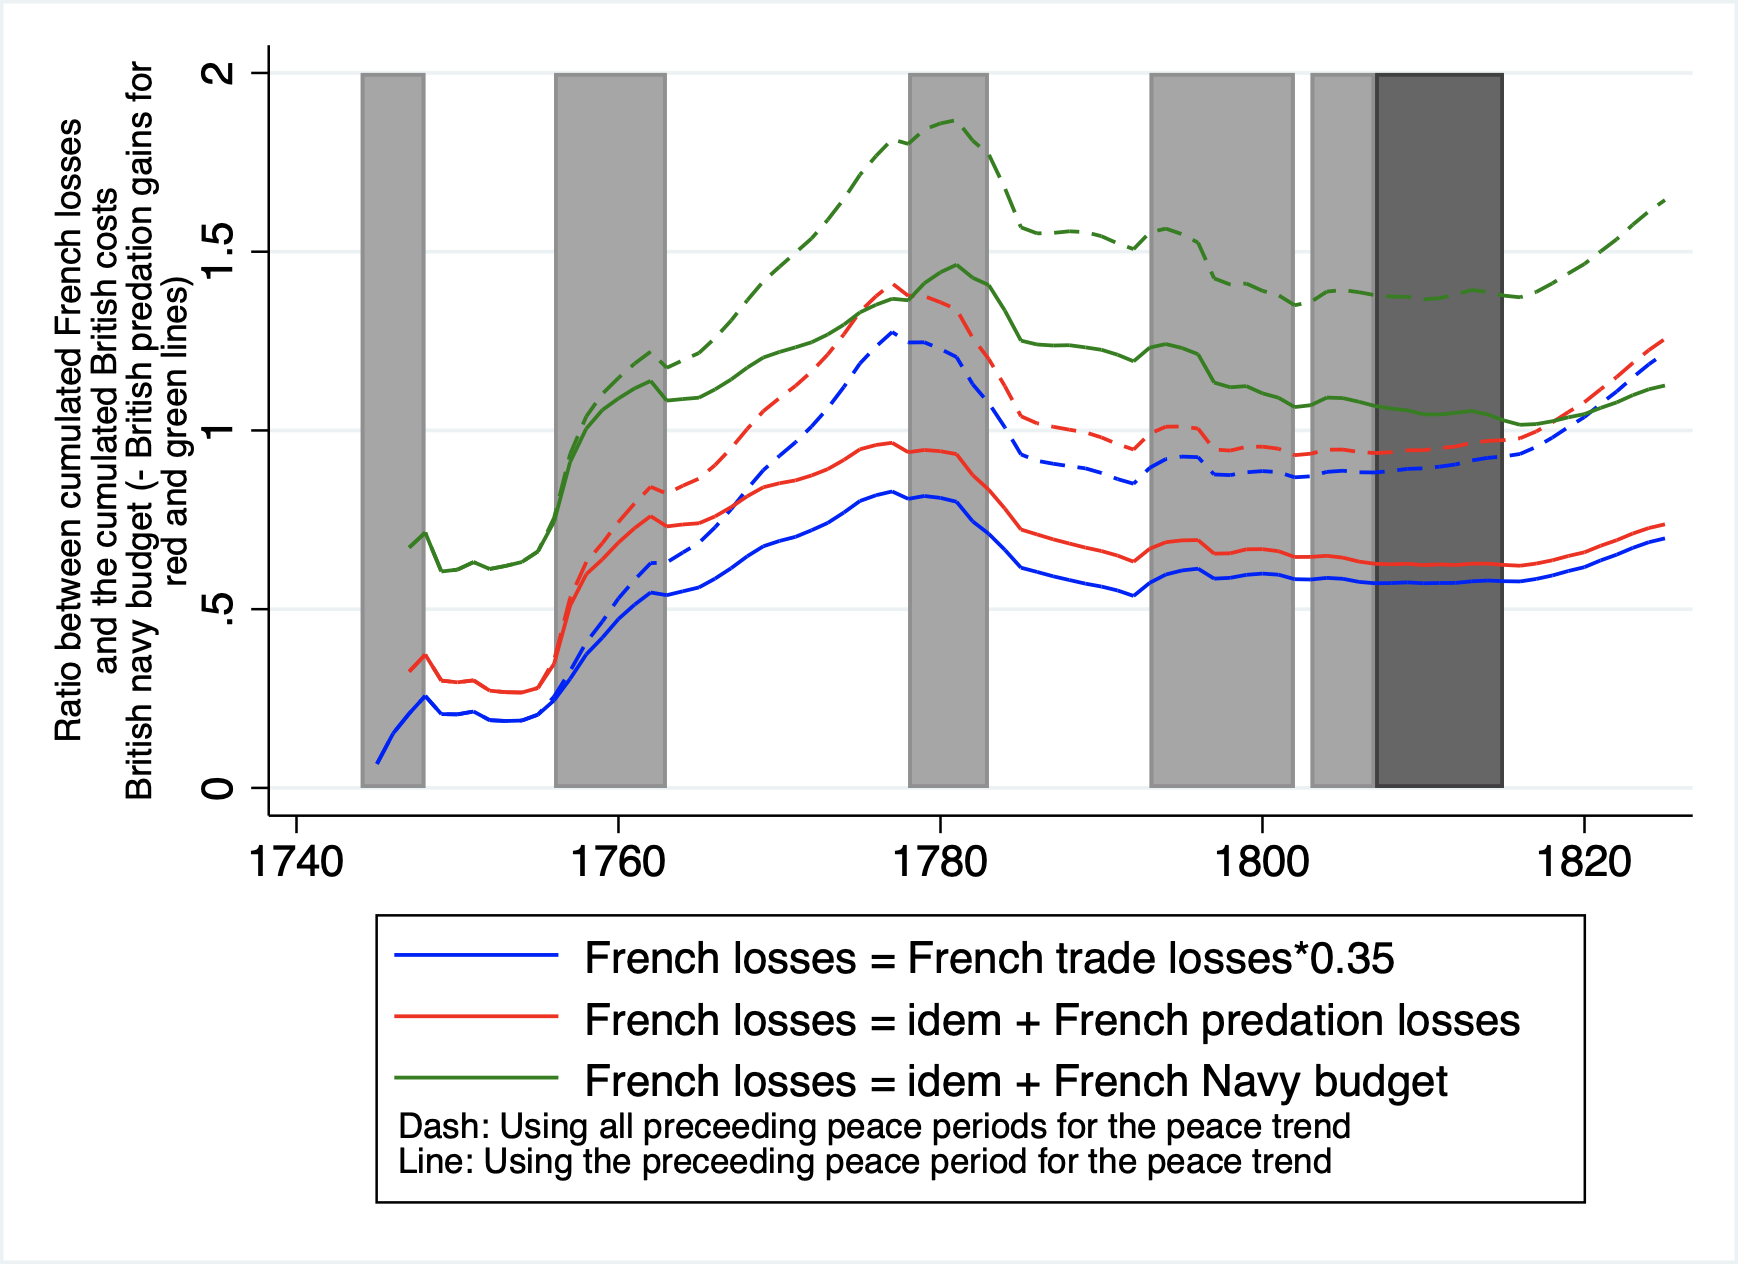
\includegraphics[scale=0.4]{Ratio_BR_Expenditures_Annual_LossH.png}
		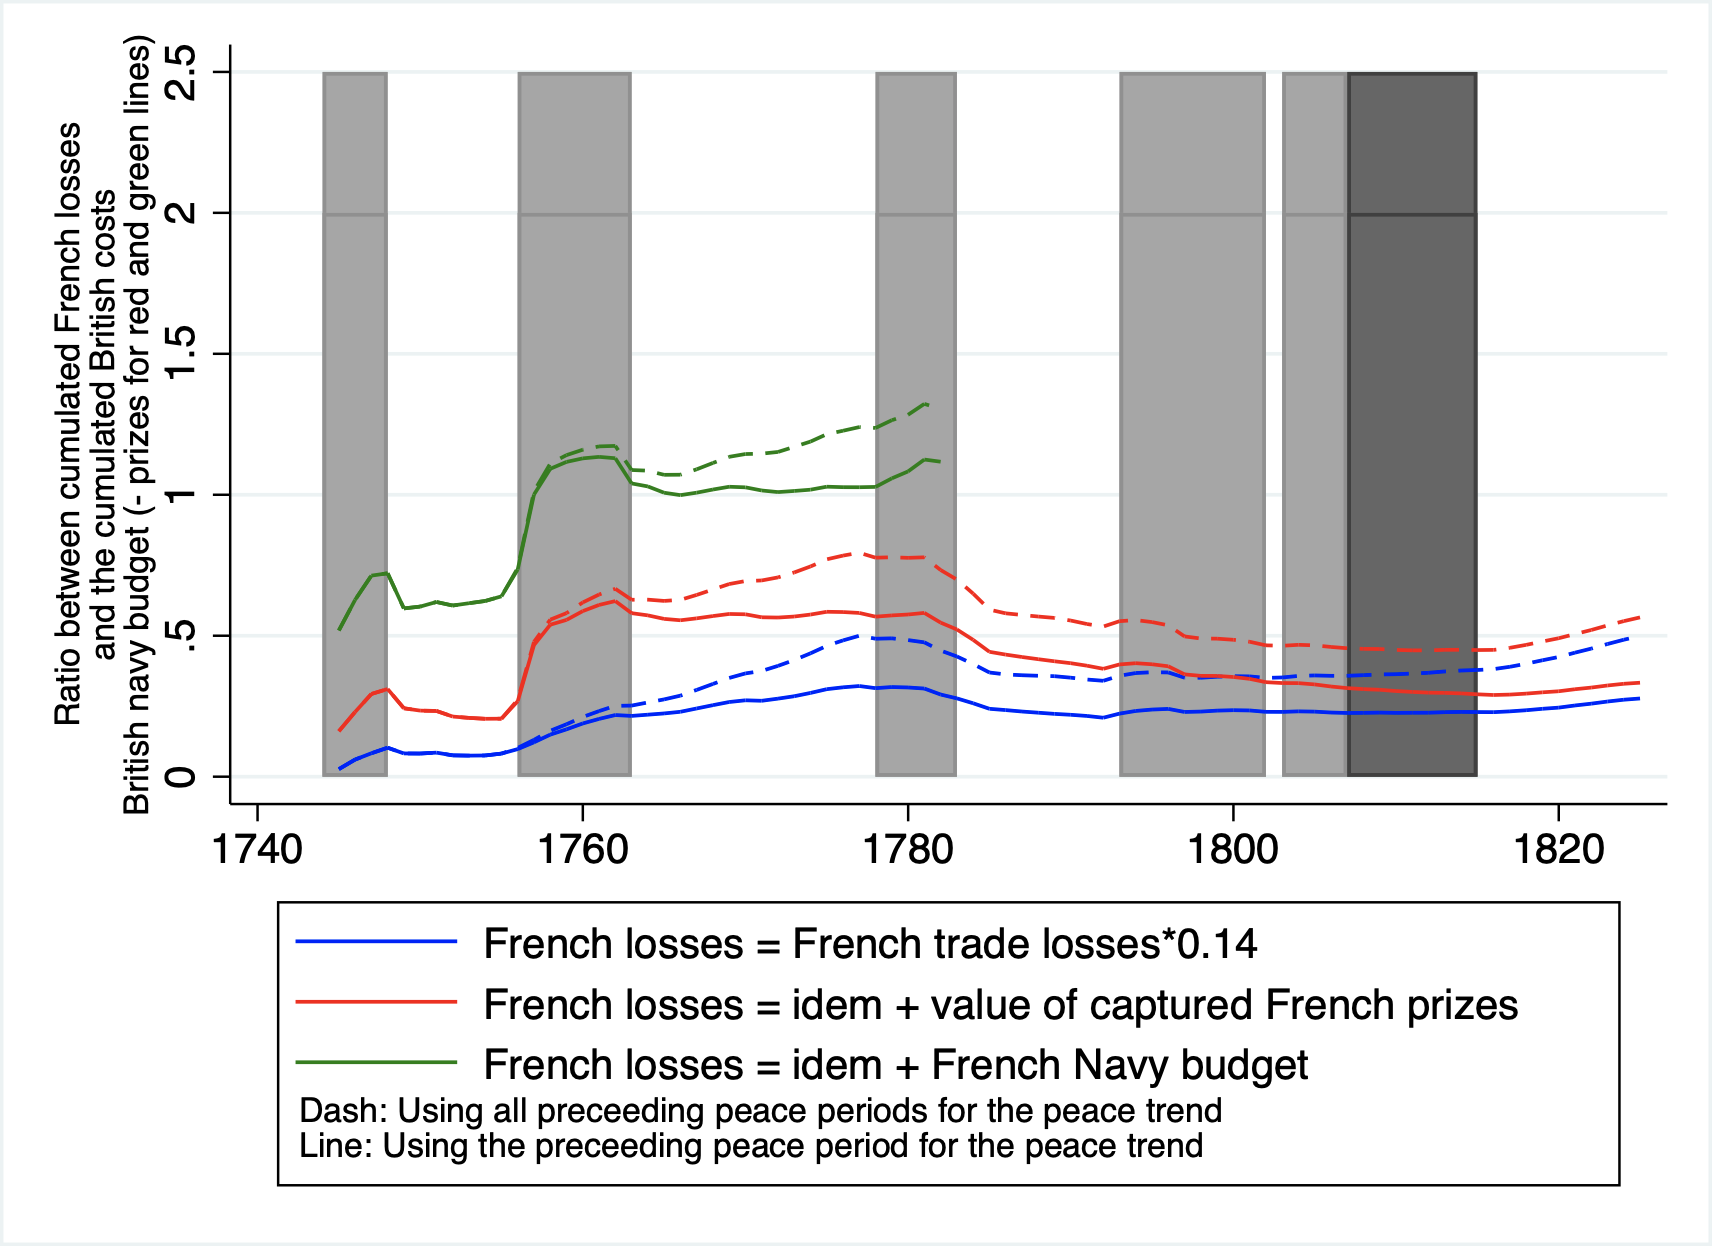
\includegraphics[scale=0.4]{Ratio_BR_Expenditures_Annual_LossL.png}
		\source{See text and \cite[pp. 570-587]{mitchell1988}}
	    \caption*{For these graphs, French trade loss are assumed to be nil for 1783-1786, 1790-1791 and at the 1797 level for 1793-1796}
	\end{figure}
\end{center}





\subsection{Explanatory variables}

With basically four observations, as we observe four wars, one cannot hope to uncover robust statistical relationships. Still, we can check the coherence of usual explanations for the disruptions of French trade.
\subsubsection{Destruction of French shipping}\label{section:DestructionofFrenchshipping}
French merchant ships were directly affected by the action of British privateers and the Royal Navy. 
\cite{Hillmann2011} estimate that British privateers intercepted about 11.5 percent of French merchant ships and 4 per cent of the value of French overseas trade during the War of Austrian Succession, the Seven Years War and the War of American Independence. 

\cite{Starkey1990} provides the number of prizes condemned as legal by the High Court of the Admiralty in London, both from privateers and the Royal Navy from 1702 to 1785. 
Prizes are a good measure of the pressure exerced on trade, as British state limited its alternative, ransoming, more and more drastically from 1744 (see \cite{Hillmann2011}, p. 734 ).
Privateering activity became marginal during the Revolutionary \& Napoleonic Wars because the development other profit alternatives.
Thank to data provided by Henning Hillmann (coming mainly from records at the PRO High Court of the Admiralty archives and underlying \cite{Hillmann2011}), we can compute an approximation of the number and the nationality of prizes captured by privateers up to 1809. Finally, \cite{Benjamin2009} provides a chronology of prizes taken by the Royal Navy in the sample first gathered by \cite{Hill1998}. Putting these data together yields Figure \ref{Prizes}.
Another measure of the the British excerciced on French trade exerciced comes from data on prize goods imported in Great Britain up to 1800 (see Figure \ref{Prize goods imports})).

\begin{center}
	\begin{figure}[H]
		\caption{Ships captured by Great-Britain}
		\label{Prizes}
		\centering
		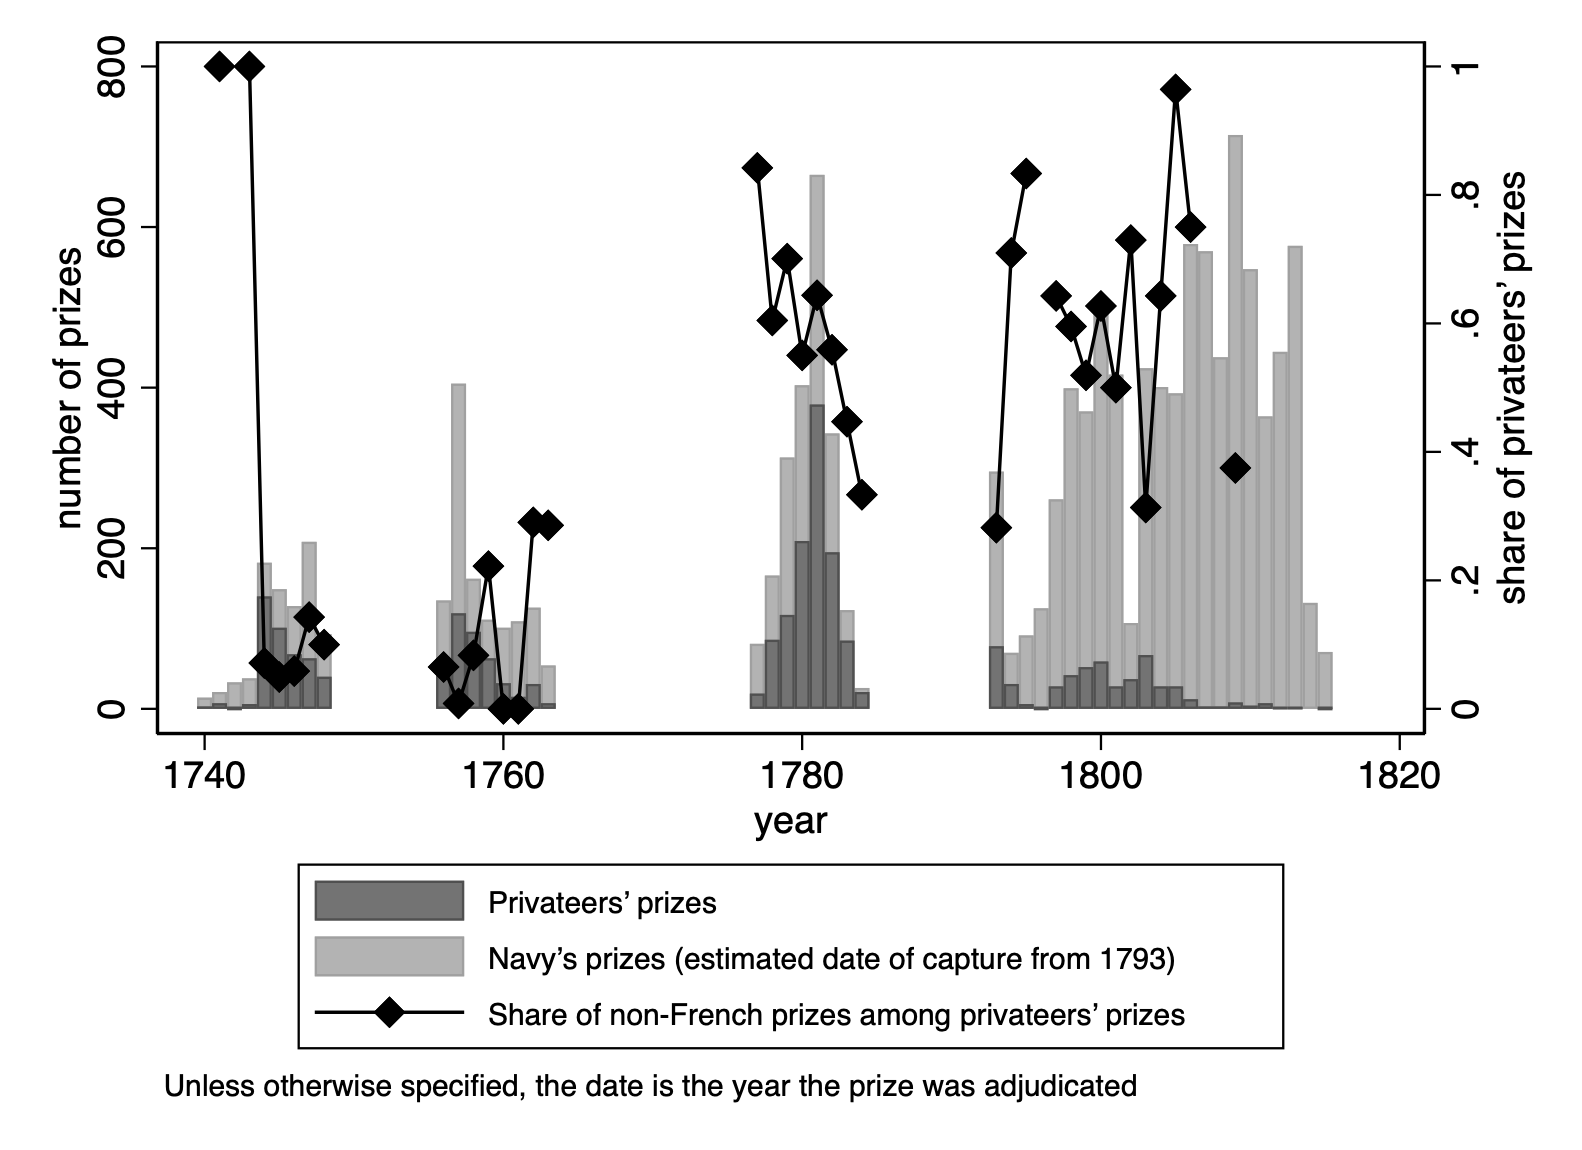
\includegraphics[scale=0.7]{Prizes.png}
		\source{\cite{Starkey1990}, data provided by Hennening Hillmann, underlying \cite{Hillmann2011} and  \cite{Benjamin2009}, based of the work done by Hill for \cite{Hill1998}}
	\end{figure}
\end{center}

\begin{center}
	\begin{figure}[H]
		\caption{Prize goods imports in Great-Britain}
		\label{Prize goods imports}
		\centering
		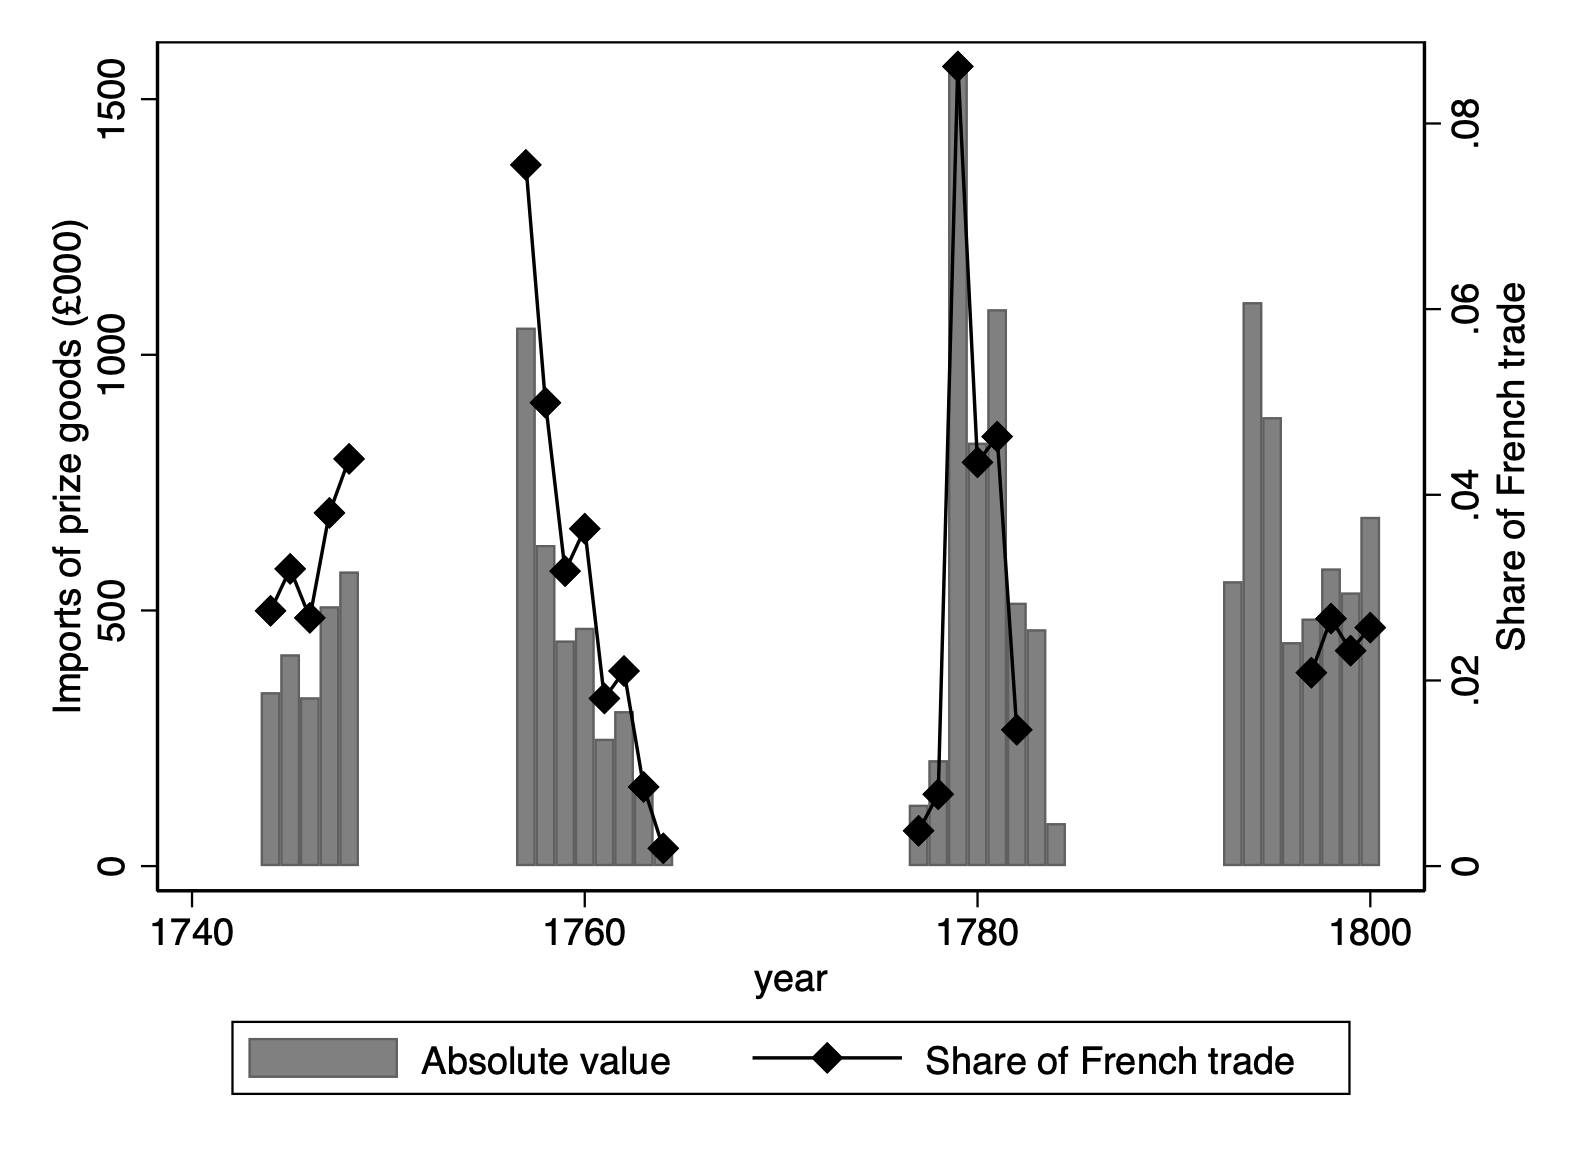
\includegraphics[scale=0.7]{Prizes_imports.png}
		\source{\cite{Ashton1960}}
	\end{figure}
\end{center}


Both these variables aroud outcome measures. 
The numbor of prizes could be declining because French ships stop sailing rather than because the probability of capture becomes smaller. A better measure of the direct naval threat might be naval supremacy.


\subsubsection{Naval supremacy}
Instead of the outcome variable, The first explanation is that naval supremacy by itself has an effect on trade.
A larger naval supremacy meant that Britain could blockade French ports and capture French ships in a more efficient way.
À CHANGER
To verify this, we use the number of warships available to France, France and its allies, Great Britain, Great Britain and its allies and neutral as provided in \cite{Modelski1988}, as a proxy for naval supremacy.
Compared to the discussion in section \ref{historical_summary}, we also track the war status of Denmark, Russia and Sweden which were sizeable naval powers during that period.
Figure \ref{naval_supremacy_ratios} reports the ratio of France over Great Britain, France and its allies versus Britain and its allies and France, its allies and neutral countries versus Britain and its allies.
Suprisingly, the most favorable war for France and its allies was the Seven Years War, thanks to the French support by Sweden and Russia, even thought there was no common naval action.
There also are some spikes during the Napoleonic Wars.
The least favorable war was the Austrian Succession War. 
This is paradoxical, as it appears that French trade suffered most when its navy, and the navy of its allies, was at the highest.
There are no simple relationship between this naval supremacy ratio and the loss function. 
\begin{center}
\begin{figure}[H]
\caption{Naval Supremacy Ratio}
\label{naval_supremacy_ratios}
\centering
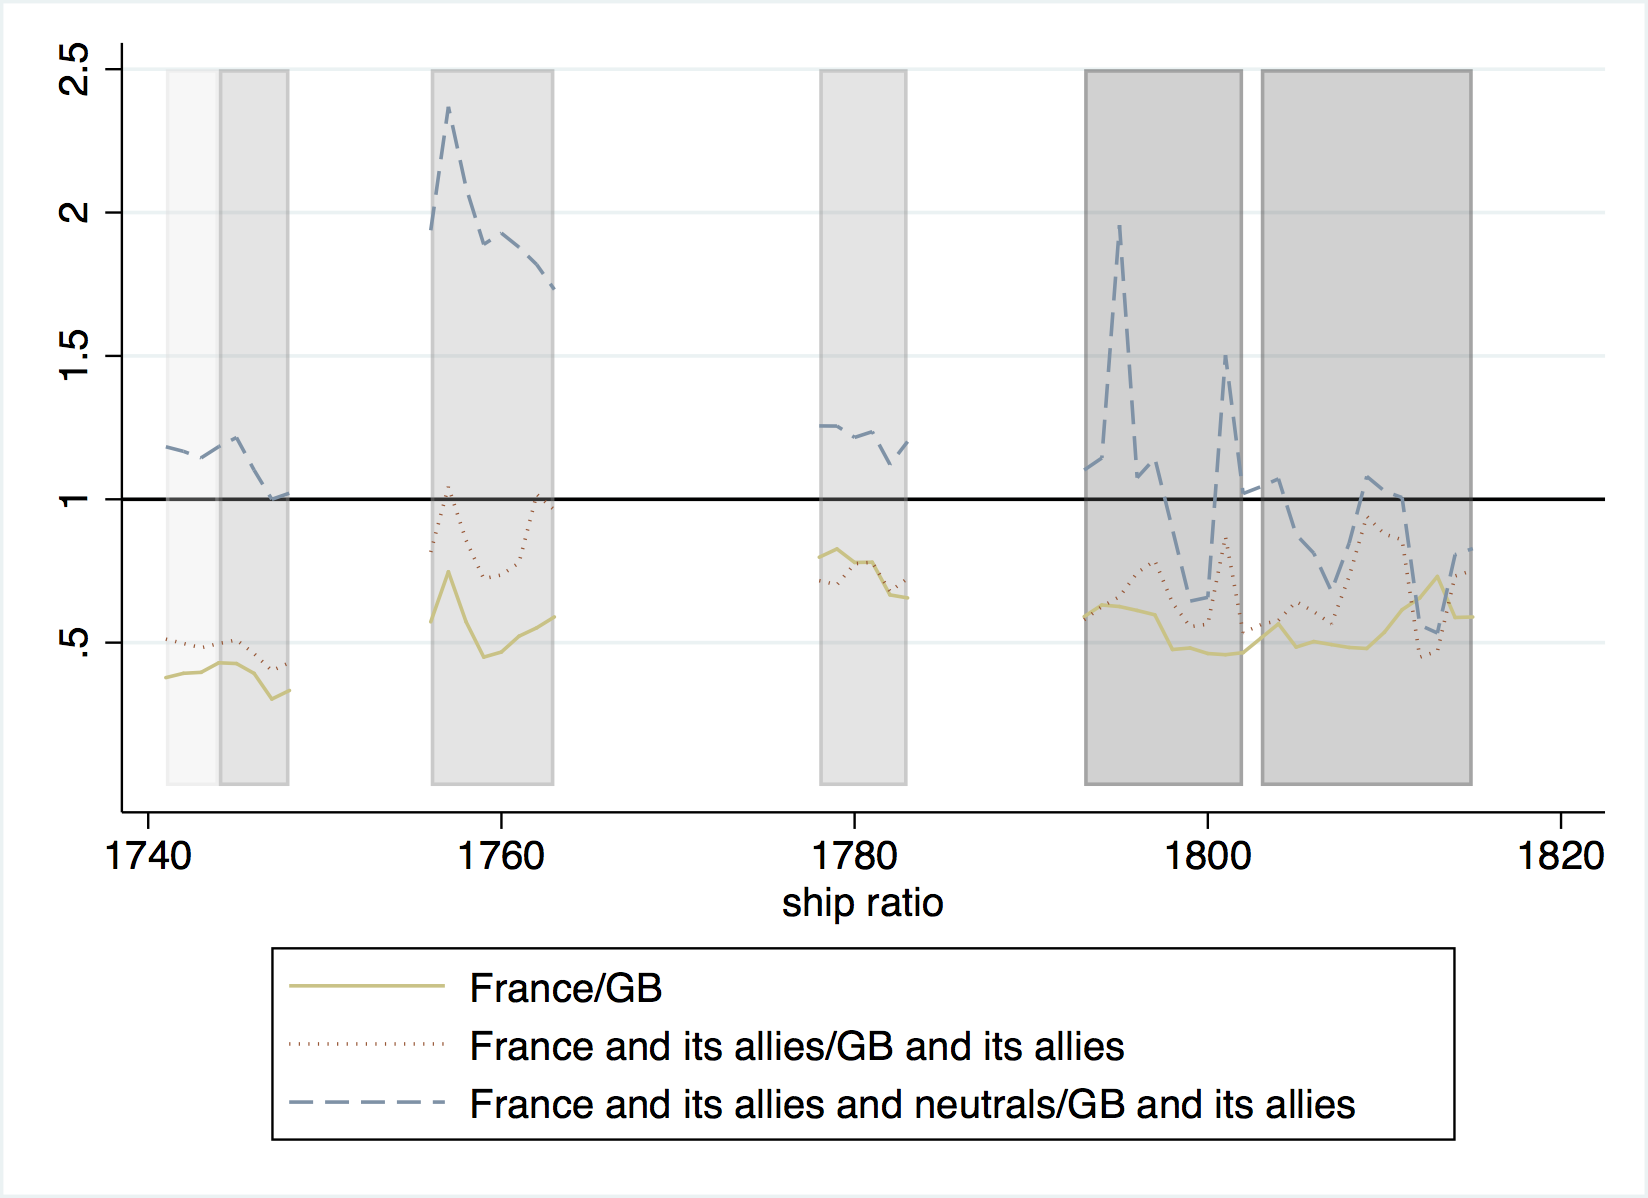
\includegraphics[scale=.51]{naval_supremacy_ratios.png}
\end{figure}
\end{center}
\subsubsection{Measure of colonial power}
West Indian French colonies were a major source for production of sugar and coffee, which were widely imported and then re-exported by France to other European countries. The loss of these colonies was bound to be disruptive for French trade, as it reduced imports and re-exports. 
We consider as colonies Guadeloupe (taken by the British in 1760, given back in late 1763 ; taken again in 1811, given back in 1816), Martinique (never lost), Saint-Domingue (revolt in 1793, partly integrated back to the French trade network in 1796, independent for good after 1804), Maurice (lost for good in 1811), Réunion and the Indian trade posts (lost in 1811, back in 1815), French Guyana (lost in 1810, back in 1817) and Tobago (lost in 1793). We construct a colonial loss measure weighting each colony by its share in French colonial imports in 1788 (TOFLIT18 data - Saint Domingue weights 75 percent, Martinique 11 percent, Guadeloupe 6 percent, India 3 percent and all the other are smaller), which is equal 1 in 1788 (considering France had its "complete" empire) and gets reduced by an amount proportional to the share of trade whenever a colony is lost. \\
An additional comment needs to be made on Saint Domingue, which was the major source for colonial goods for France. 
The revolt of the slaves in Haiti was a long and bloody episode and sugar production was lost well before independence was ultimately acquired.
We have coded it as "lost" between 1793 and 1795, when the revolt started, and production was mostly destroyed or fields burnt.
In 1796, order was partly restored and a portion of the plantation were being cultivated normally, and only 1805 Haiti became independent and the production was lost completely.
Guadeloupe was also important for its sugar production and was lost to the British between 1759 to 1763, as it is visible from the decrease of the index in the graphs, and between 1810 and 1816.
Finally, Martinique was controlled almost continuously by the British, from 1794-1815, to be traded back to France, after the Napoleonic Wars.
Figure \ref{colony_loss} shows the evolution of the colony loss measure.

\begin{center}
\begin{figure}[H]
\caption{Colonial empire loss}
\label{colony_loss}
\centering
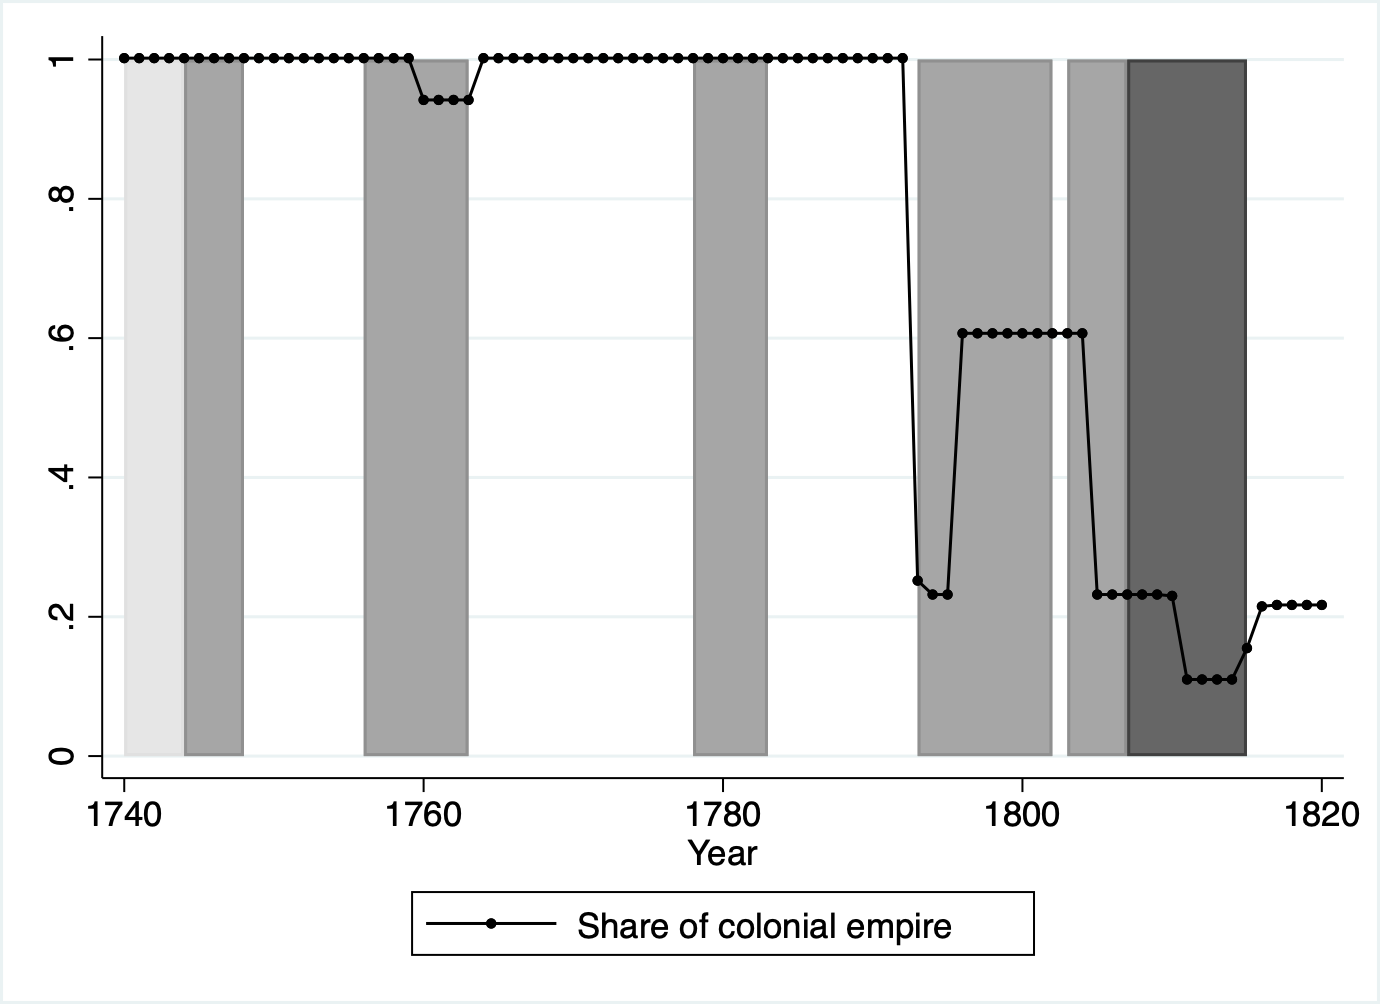
\includegraphics[scale=.51]{colony_loss.png}
\end{figure}
\end{center}
Again, the link with the trade loss measure is not obvious. It works well for the Revolutionnary \& Napoleonic Wars: a large part of the empire was gradually lost in that period. But the colonial loss of the Seven Years War were minimal (Canada was not an important trade partner for France) and do not seem to justify the larger trade loss during that period.
It is interesting to remark that in 1814, the Restauration was keen to re-create the colonial system from the late eighteenth century.
This included the re-establishment of the \textit{Exclusif} and reconquest of St-Domingue or the establishment of some substitute colony (\cite{Todd2011}).
In a secret clause of the 1814 peace treaty, Great-Britain pledged not to hinder the re-instauration of French sovereignty on St-Domingue (\cite{Schefer1907}).
That seems hardly compatible with the idea that the loss of colonies was a necessary nail in the coffin of French trade.

\subsubsection{Neutral policy}
While trying to destroy foe's shipping, the way the Neutrals were treated was important. First, they could benefit from providing goods that were not available anymore because of war ()\cite{Hedberg2015}). Beside trade diversion, the merchants from belligerent countries used a number of devices to "hide" their cargo as neutral cargo and continue trade (for example, see \cite{Carriere1973,Schnakenbourg2013,Schnakenbourg2015}).

During war, enemy cargo could be seized. But the crux of the matter was the definition of "enemy cargo". It obviously included merchandises transported by enemy ships, so one would use neutral ships.
Shipping between a nonbelligerent country and a non-blockaded port in France was allowed by the rules of war and Great-Britain, provided that both the ship and the goods belonged to neutral merchants.
Neutral shippings to actually blockaded ports could be seized, but not that to other enemy ports \citep[p. 112]{Schnakenbourg2013}.
The practice of seizing neutral ships can be seen in Figure \ref{Prizes_nationality}.
Presumably, some ships flying a neutral flag were declared "French" at the High Court of the Admiralty.
Still, it also adjudicated that some neutral ships were fair prizes (e.g. Dutch ships before the Fourth Anglo-Dutch war that started in 1781 and US ships during the 1790s).

\begin{center}
	\begin{figure}[H]
		\caption{Nationality of non-French British prizes}
		\label{Prizes_nationality}
		\centering
		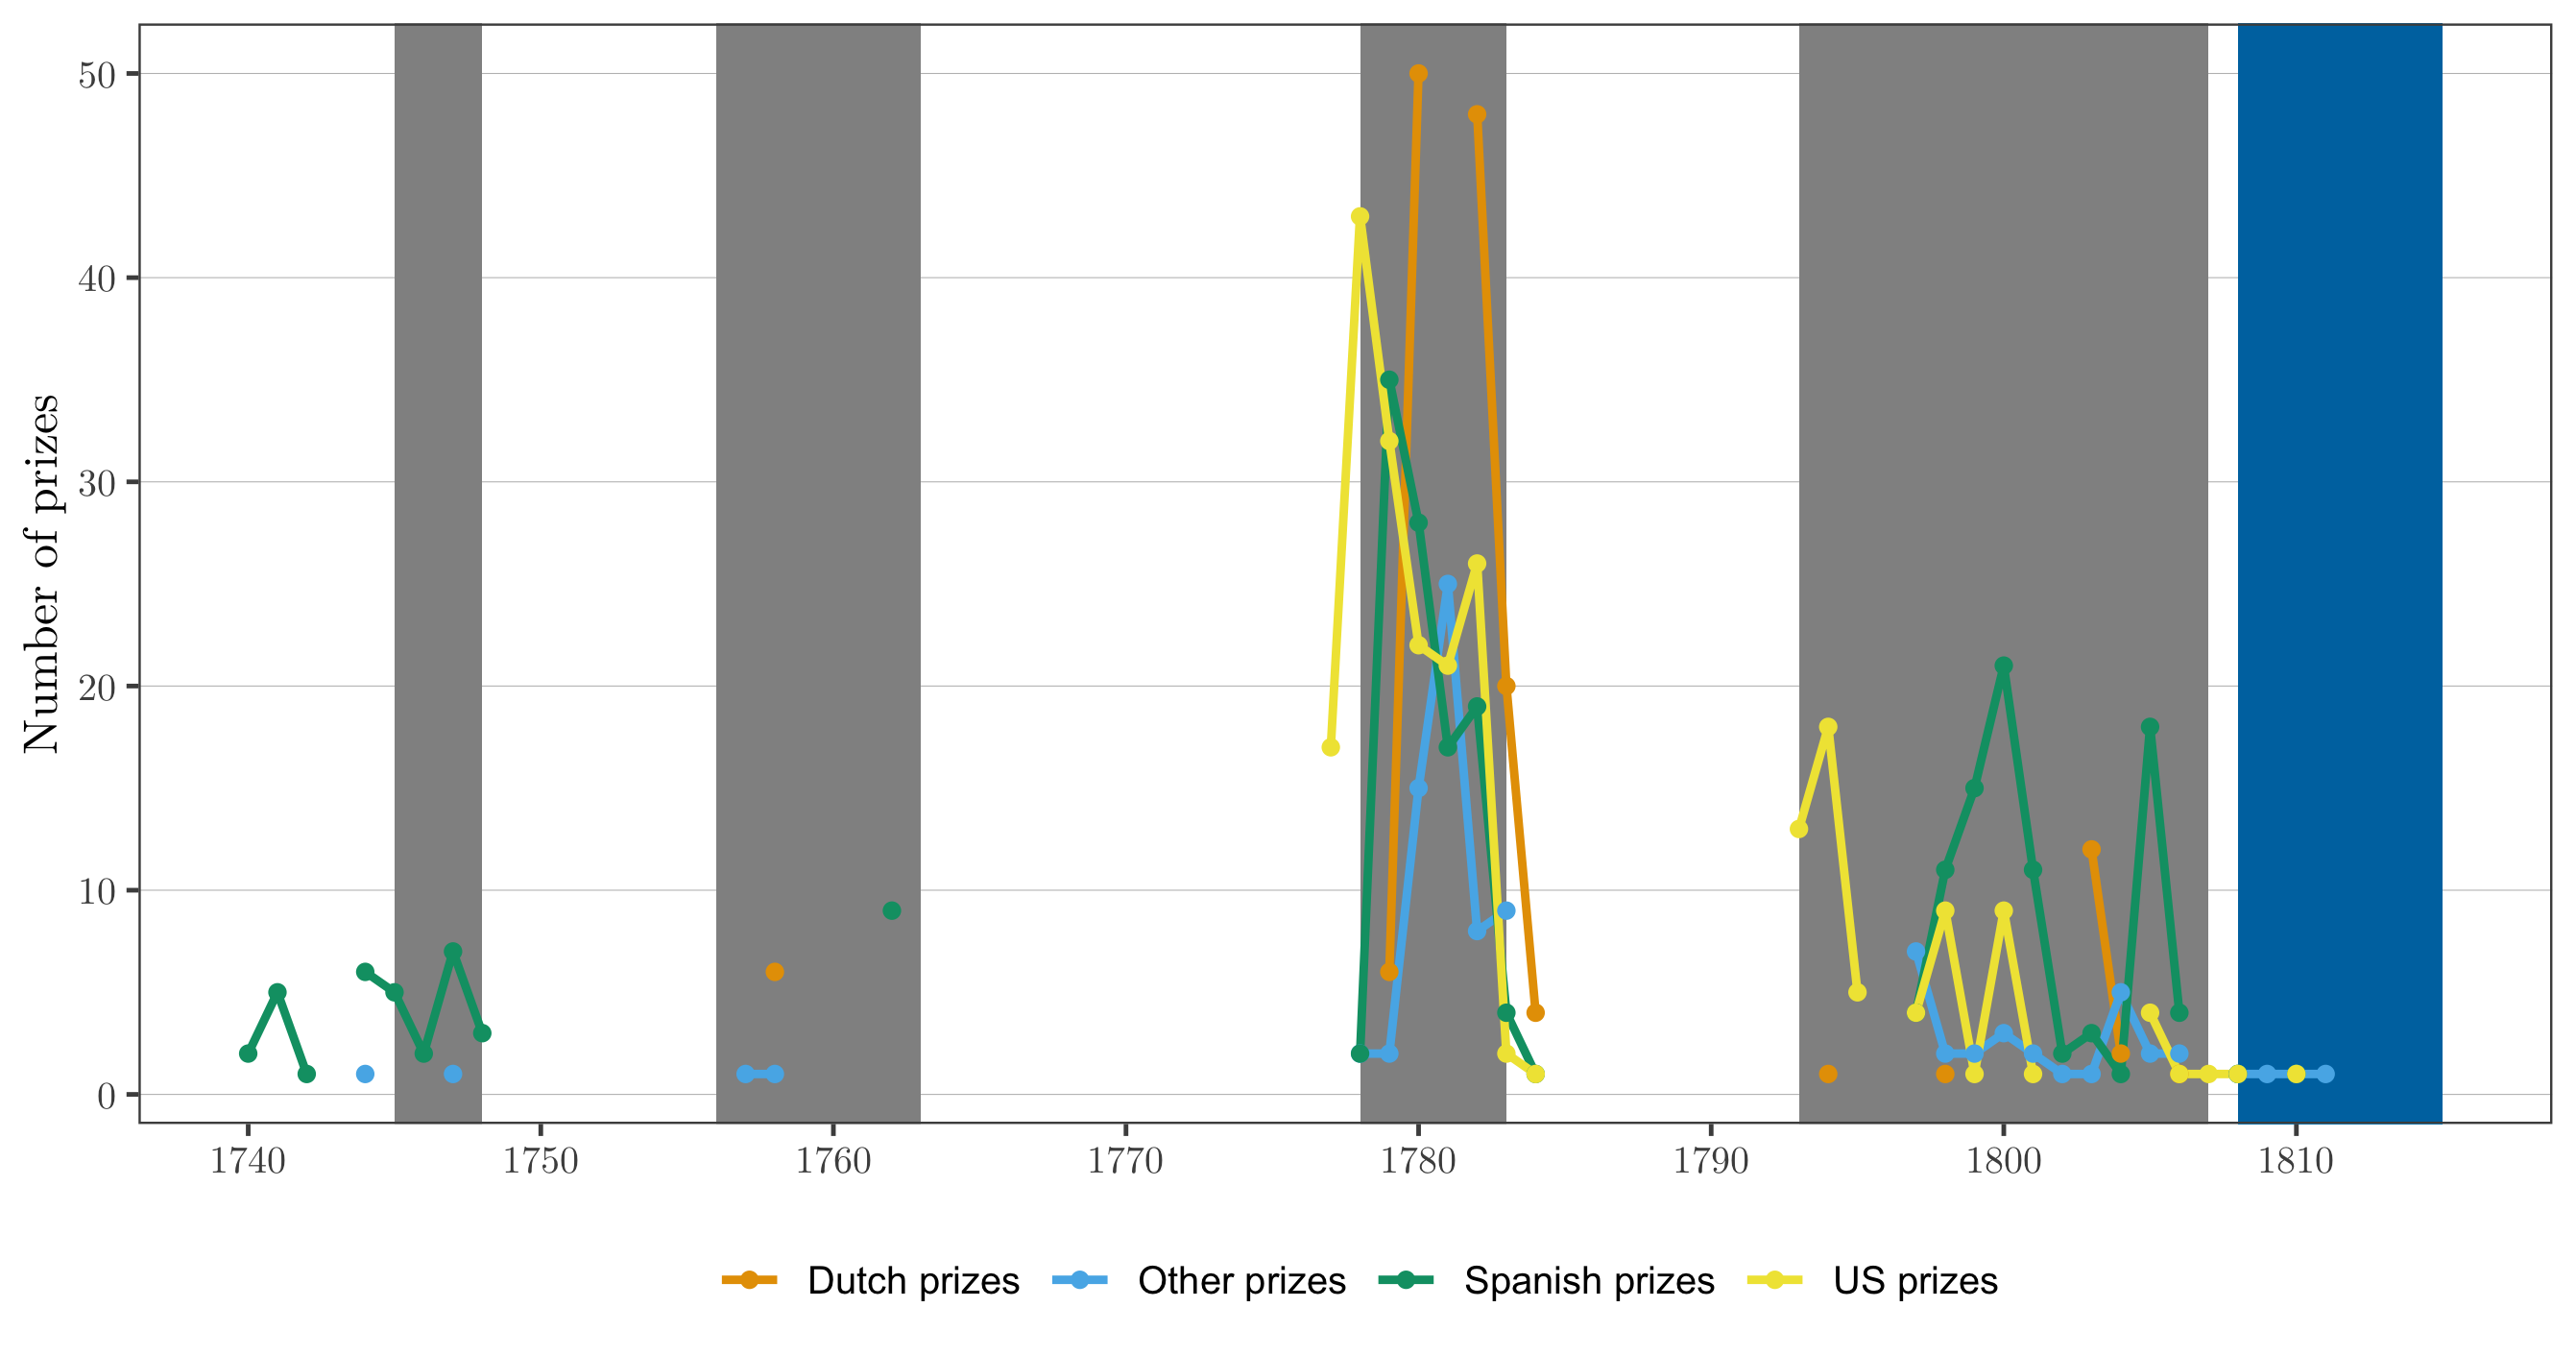
\includegraphics[scale=.51]{Prizes_nationality.png}
		\source{See Figure \ref{Prizes}}
	\end{figure}
\end{center}


During the War of Austrian Succession, the British did not fight neutral trade very strongly and allowed neutral countries to continue trading though they were prohibited to carry "enemy cargo" (i.e. cargo owned by the enemy). But there was no way to check anyway, as neutral ships would not yield to inspection, especially when they were escorted by neutral warships (they had claimed from the seventeenth century the "right of convoys", "that is, immunity from search for neutral merchant vessels sailing under the convoy of a warship of the neutral"  \citep{TheEditorsofEncyclopaediaBritannica2014} .
For example, French colonial goods would be taken from the French West Indies to the Dutch West Indies (e.g. St. Eustache) and then brought to Europe.
As the cargo was not coming directly from French West Indies, it was not deemed "enemy cargo". 
During the eighteenth century, belligerent countries - especially Great Britain - tried to  close off these ways for French trade to continue thanks to neutral shipping.
In 1756, during Seven Years War, the British decided to put an end to just aforementioned practice and introduced the \textit{Doctrine of Continuous Voyage} along with the \textit{Rule of War of 1756}, that stated that the very beginning of the journey and the very end should be taken into account to determine the nationality of the cargo.
They also claimed the right to seize neutral shipping to look for contraband (and exercised it).
Also, they forbid neutrals, in time of war, to enjoy a trade from which they were barred in time of peace. As the French colonies were under the regime of the \textit{Exclusif} (\cite{Tarrade1972}), and that all their trade had to be conducted by French ships, that basically barred neutrals from trading with the French colonies.
This had a considerable impact on French trade, which was heavily relying on Dutch ships to transport colonial goods.
It also created great discontent among neutral countries. They were not able to enforce their rights efficiently until 1780, when, finally, Russia, Denmark and Sweden created the \textit{League of Armed Neutrality}.
The latter allowed them to defend their interest at least for the time of the War of American Revolution.
The idea was that neutral ships traveling under the protection of neutral warships were not to be inspected as the absence of "enemy cargo" was guaranteed by the neutral sovereign (\cite{Schnakenbourg2013}, p. 121-125).
This experiment however did not have a long lasting success and was finally put to an end in 1783 with the treaty of Paris, when Catherine of Russia renamed it the \textit{Armed Nullity}\footnote{The number of vessels Russia, Denmark and Sweden owned combined were still less than the entire British navy, therefore this league was bound to be weak from the very beginning.} \citep{Griffiths1971}.
Still, Ancien Régime France was active at protecting the rights of neutral shipping, as it saw it as mean to continue its trade during war years (\cite{Schnakenbourg2013}, p. 129).
In 1784, France gave the West Indies island of St. Barthelemy to Sweden partly to encouraqe neutral trade during wars (\cite{Schnakenbourg2013}, p. 326).

  
The situation was very different during the Revolutionnary \& Napoleonic wars.
The United States were a new independent actor in international trade.
They played a very important role in "neutralizing" French trade \citep{Marzagalli2005,Marzagalli2015}), but also as intermediaries between Great-Britain and Spanish America (\cite{Cuenca-Esteban2014}).
But considering the dynamism of their economy, they were not as easy to dismiss when peace returned.
Still, their shipping income was divided by four between the high points of 1807 and 1811 (40 Million US\$) and the 1820s (less than 10 Million US\$) \citep[tables A-4 and B-2]{North1960}.
Another change was that France become more and more hostile to neutral shipping in trying to isolate Great Britain.
With both countries trying to curtail neutral shipping, the system through which it was an objective ally of French trade crumbled down.
In 1793, with the outburst of the French Revolution and, subsequently, the Revolutionary Wars, most British goods were prohibited in France.
As a response, the British adopted a policy for blockading the coast of France and, subsequently, both countries took action against neutral shipping.
A year later, Denmark and Sweden attempted again to enforce their rights by creating a \textit{Second League of Armed Neutrality}, which was joined by Russia and Prussia in 1800.
No later than 1801, though, the British blockaded them (with the exception of Prussia) and bombed Copenhagen to end the League for good.
In 1806, things worsen even further for neutral countries, when Napoleon enacted the Berlin decree, which provided the basic structure of the Continental System.
The provisions of the Berlin Decree included: (1) prohibition of all trade with the British; (2) all British subjects in French-occupied areas were prisoners of war and their property was "fair prize"; (3) all trade in British goods was prohibited and all goods from England and her colonies were fair prize (and one-half their value was to be used to indemnify French merchants for losses to the British); and (4) no ships coming from the ports of Britain or its colonies would be permitted to use any port on the Continent \citep{Davis2006}.
Britain responded to this policy with a related Order in Council, which required that neutral vessels call at a British port before proceeding to the continent, hitting at neutrals such as the United States, as well as France \citep{Davis2006}.
The United States, were, at the time, the biggest neutral country whose trade was suffering because of the Blockade and, as a consequence, they attempted to fight back.
They first enacted, in 1807, an Embargo Act directed against trade with both France and Britain, which was followed by the Non-Intercourse Act of 1809, and finally, after failure of both provisions, by a war against Britain.
The United States had no better luck than France in the war, which was ultimately won by British, and caused considerable decline in trade for both sides.
The situation started to unravel only around 1810, when Russia pulled out of the Continental Blockade, pushing Napoleon to attempt an invasion, which ultimately led to his final defeat, but put an end to the Blockade System and to the threat for neutral trade.

Based on these facts, we have created a categorical variable that can take two values; 0 when there was no policy against neutral shipping in wartime and 1 when neutral cargo became "fair game". 
%three values; 0 if only enemy cargo were fair game, 1 if enemy cargo on neutral ships were fair game, 3 if any good from enemy territory  were fair game.
As a consequence, for this variable, we would expect a positive effect; the higher the value, the stricter the policy and the bigger the loss.
The table \ref{neutral_policy} reports the value of this variable overtime.
Table \ref{summary} reports a summary of all expected effects of the independent variables.


\begin{table}[H]
\centering
\caption{Measure of neutral policy}
\label{neutral_policy}
\begin{tabular}{ll}
\hline \hline
Period & Neutral policy variable  \\ \hline
1741-1755 & 0                  \\
1756-1779 & 1       \\
1780-1789 & 0                 \\
1797-1820 & 1                 \\
\hline 
\end{tabular}
\end{table}

\begin{table}[H]
\centering
\caption{Summary of expected effects}
\label{summary}
\begin{tabular}{ll}
\hline \hline
Explanatory Variable & Expected Effect  \\ \hline
Loss of colonies & \textbf{-}                  \\
Naval Supremacy & \textbf{-}                 \\
Treatment of neutral countries &       \textbf{+}      \\ \hline 
\end{tabular}
\end{table}


This variable, such as it is, is well correlated with the trade loss function. This was moderate during the Seven Years War and after it and large during the Revolutionary and Napoleonic Wars.
This is hardly a statistically convincing argument, but it works better than the other two stories. 
There are two additional arguments to present.
Figure \ref{Number_of_protagonists} shows that there is a polarization of French trade partners duning the Revolutionary \& Napoleonic Wars.
War engulfed the whole of Europe and the only remaining neutrals trading region during the Napoleonic period was the \textit{Levant}.
It could hardly play a role by in sustaining French trade.
Figure \ref{loss_by_war_status_XI} is constructed by computing the mean country-specific trade loss function by war status. The trade loss function has been computed based on all preceding peace periods.
We have both a trade-weighted measure and a non-trade weighted measure.
\textit{Empereur} after 1794 had to be excluded, as the territorial change was too large (trade was mainly with current Belgium before 1794 and mainly with Austria after 1794).
\textit{Hollande} after 1814 had to be excluded as well as it included current day Belgium from 1815.
The negative trade loss number for trade with foes in 1787-1789 is a tribute to the large effect of the Eden treaty.
Notice that trade with neutral countries does not recover at all after the Seven Years War and hardly recovers after the Revolutionnary \& Napoleonic Wars. 

\begin{center}
\begin{figure}[H]
\centering
\caption{Trade loss by war status}
\label{loss_by_war_status_XI}
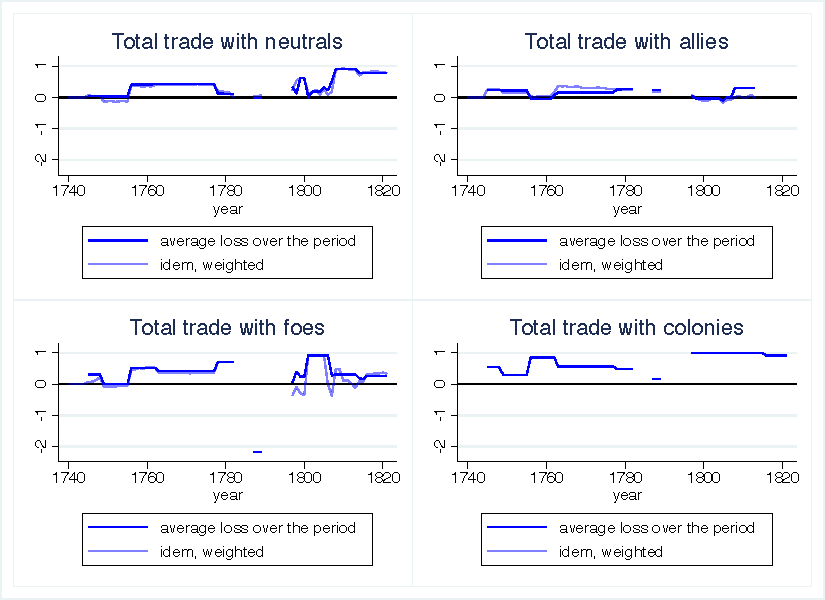
\includegraphics[scale=1.2]{loss_by_war_status_XI.pdf}
\end{figure}
\end{center}
Both  Figure \ref{Number_of_protagonists} and Figure \ref{loss_by_war_status_XI} suggests that trade with neutral is important in explaining the contrasting resilience of French trade after each of its war with Great-Britain.
To go further and understand the reason behind this behaviour, we need to look into the changing goods structure of trade during the wars.

\section{Econometric analysis}  \label{economtrics}
Before moving on to look into composition of trade we want to quantify the effects observed so far. This is not an easy task because the number of observations is limited - we only have 12 countries for 65 years in the best case - which does not leave us enough degrees of freedom to run any properly specified regression including all the variables. We have therefore opted for running a regression for each single variable of interest. We have done so for the total loss function, for the loss function broken down for neutral allies and foes and for the loss function disaggregated by country \footnote{In all those cases we have clustered the standard error by periods}. \\
We start by regressing the loss function on our index of colonial power and controlling for peace and war period. Table \ref{effects_colonial_power} shows the results. 
\begin{figure}
\centering
\caption{Effects of colonial power}
\label{effects_colonial_power}
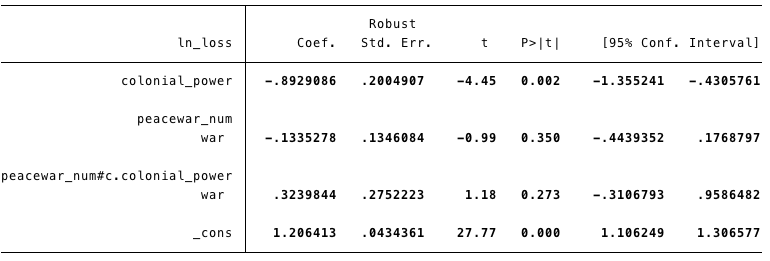
\includegraphics[scale=.65]{reg1}
\end{figure} 
Colonial power has indeed a negative and strongly significant effect on trade loss, which is to say the more of its colonies were under French control, the least is the loss in trade. The war per-se does not appear to be significantly causing disruptions, neither is the combined effects of war and colonial power (both insignificant). \\
Doing the same for naval supremacy (Table \ref{effects_naval_supremacy}) we see that in this case, none of the coefficients is significant, suggesting that there is no direct link between lost trade and the number of French ships and its allies and Britain and its allies. \\
\begin{figure}
\centering
\caption{Effects of naval supremacy}
\label{effects_naval_supremacy}
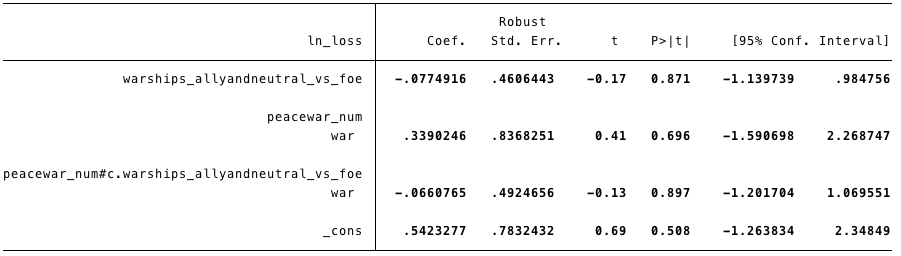
\includegraphics[scale=.6]{reg2}
\end{figure}
Finally, we repeat the same exercise for the effects of neutral policy (table \ref{effects_neutral_policy}). In this case all the coefficients are significant, with the exception of the interaction between war and neutral policy, and positive (i.e. they increase loss). It is interesting to see that the coefficient of neutral policy is higher than that for war (a simple t-test on their difference yields a p-value of 0.003). I CANNOT DO IT LIKE THIS, THEY HAVE TO BE STANDARDIZED. \\
\begin{figure}
\centering
\caption{Effects of neutral policy}
\label{effects_neutral_policy}
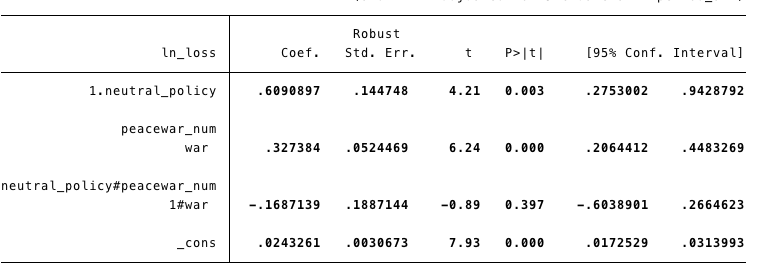
\includegraphics[scale=.65]{reg3}
\end{figure}


\begin{figure}
	\centering
	\caption{Effects of neutral policy NEW}
	\label{effects_neutral_policy}
	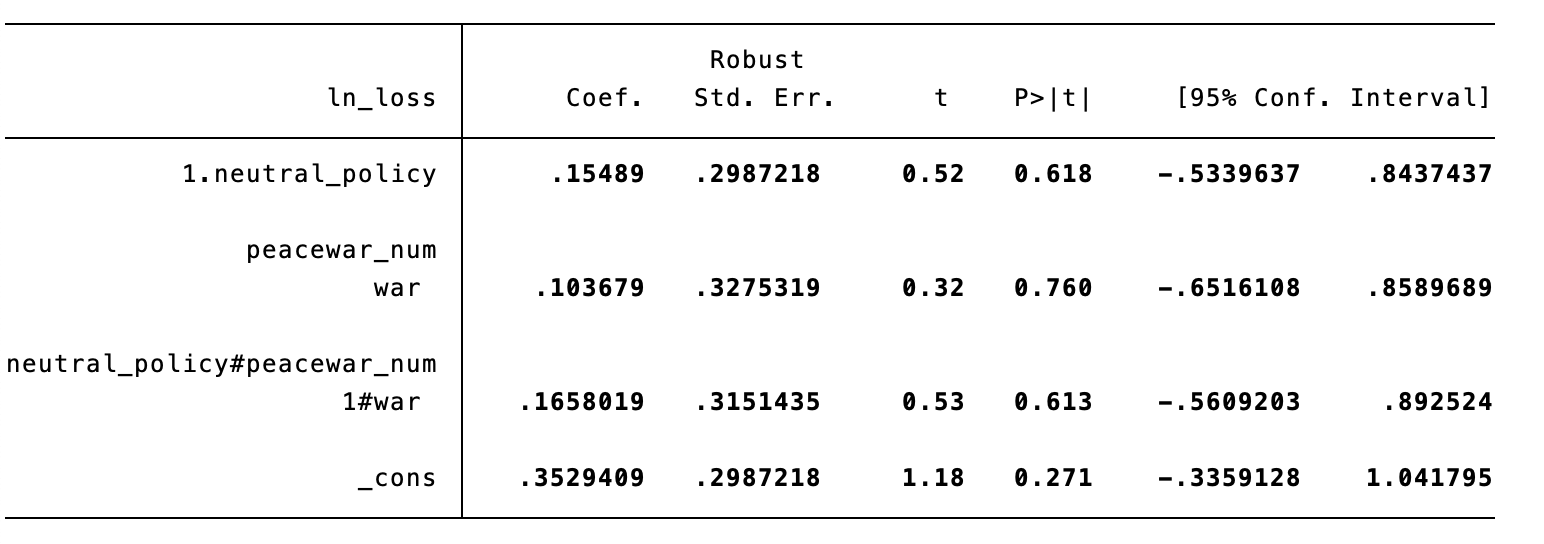
\includegraphics[scale=.65]{reg_3_Neutral_Policy_NEW}
\end{figure}

NEUTRAL POLICY HAS CHANGED QUITE A BIT

\begin{figure}
	\centering
	\caption{Effects of British prizes}
	\label{effects_neutral_policy}
	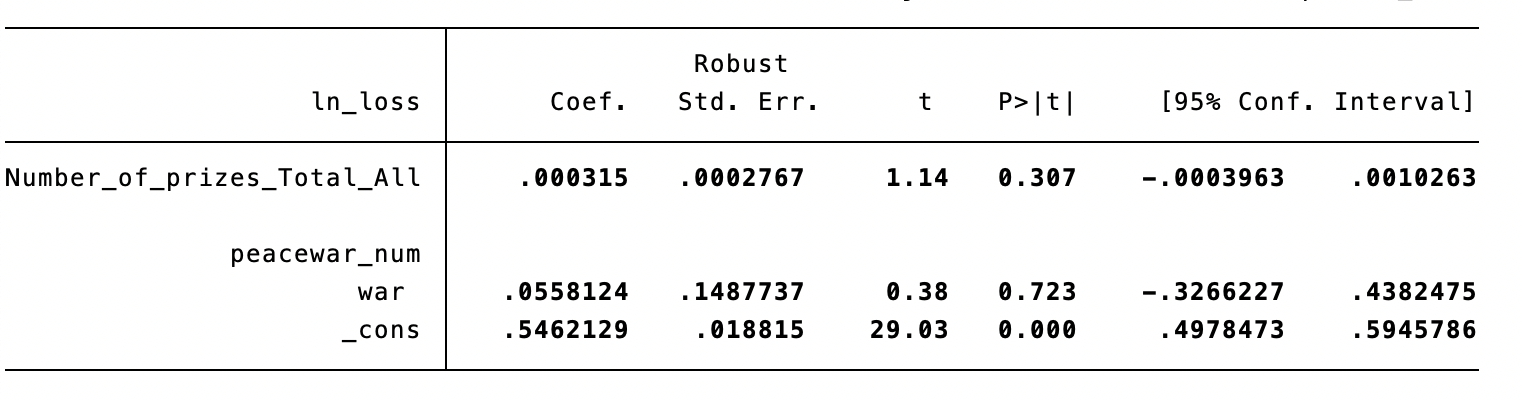
\includegraphics[scale=.65]{reg_prizes}
\end{figure}


We also run a regression on all the three coefficients together (Table \ref{effects_together}), distinguishing for war and peace in two different regressions, however we are not able to cluster the standard error in this case, because of lack of degrees of freedom. We observe here that, in time of no tough policy towards neutral countries, colonial power is very beneficial for trade (the loss is highly negative), however in war times, this coefficient loses significance and the only "driver" of the loss function is the neutral policy variable. This leads us to think that colonial power was crucial in peacetime for the flourishing of French trade, but was not enough of a shield during conflicts, if neutral trade was also targeted. 
\begin{figure}
\centering
\caption{All effects together}
\label{effects_together}
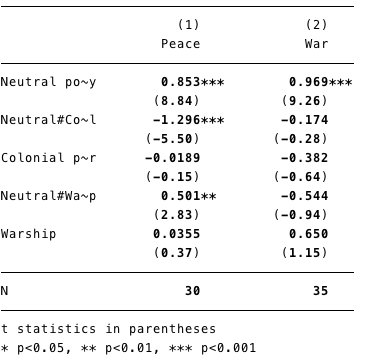
\includegraphics[scale=.8]{reg4}
\end{figure}


\begin{figure}
	\centering
	\caption{All effects together NEW}
	\label{effects_together}
	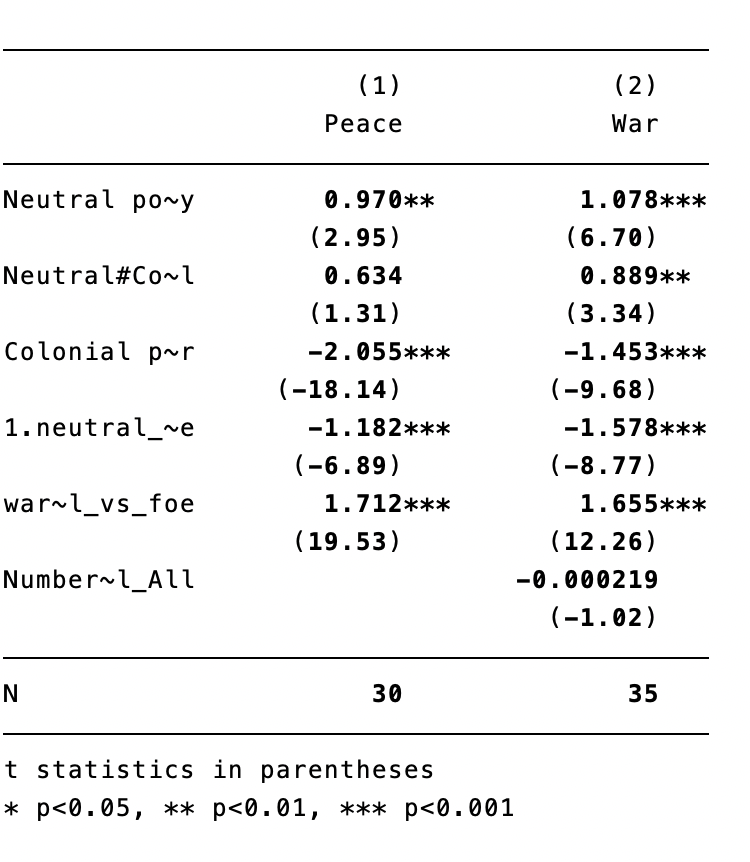
\includegraphics[scale=.8]{reg_4_all_together_new.png}
\end{figure}

Next, I go on to analysing the effects distinguishing by war status (Table \ref{effects_together_warstatus_peace} and \ref{effects_together_warstatus_war}). The idea is to try to disentangle the loss due to lost neutral trade, caused by stricter policies. In this case we gain some degrees of freedom by disaggregating the total by neutral foes and allies, but we add a dummy for  war status, and one interaction with neutral policy, so the overall degrees of freedom gain is limited. The two regressions overall do not change the picture much with respect to the results seen so far. All of the explanatory variables are significant and in the expected direction both for the peace and the war period. It is interesting to notice, again, that while they are all significant for the peace period period, only neutral policy is for the war period. This reconfirms what we had already seen in the previous analysis, i.e. that in war period the major source of trade disruption was due to crippling neutral trade. 
\begin{figure}
\centering
\caption{All effects together with war status - Peace}
\label{effects_together_warstatus_peace}
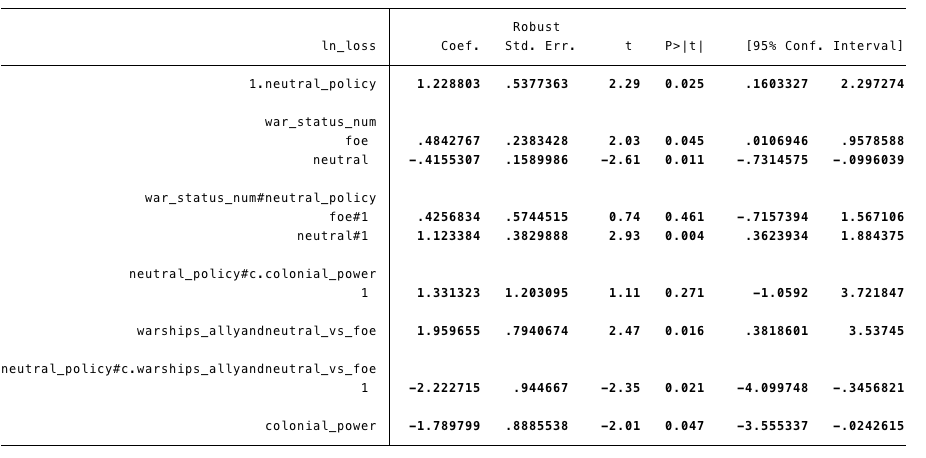
\includegraphics[scale=.55]{reg5}
\end{figure}
\begin{figure}
\centering
\caption{All effects together with war status - War}
\label{effects_together_warstatus_war}
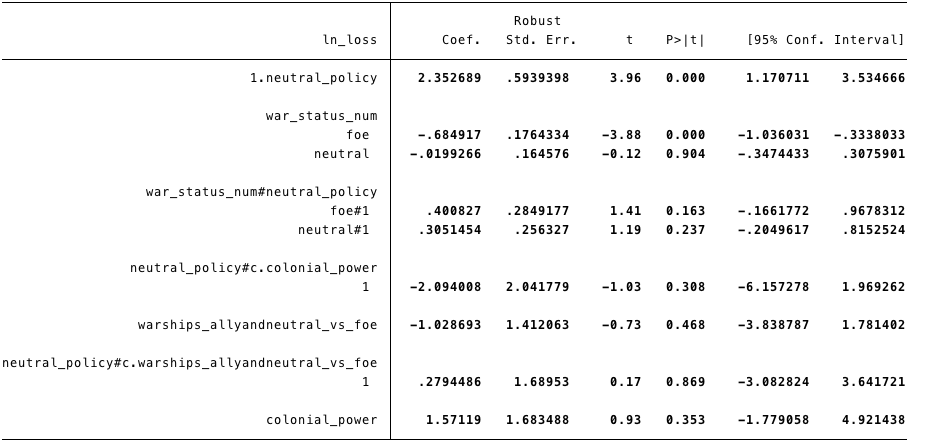
\includegraphics[scale=.55]{reg6}
\end{figure}

\section{Changing composition of trade}  \label{composition}
In this section we test whether the structure of trade was significantly different in wartime with respect to peacetime and, if so, whether the change was reversed after the end of each conflict, i.e. whether the structure of trade in the different peace periods remained unchanged. 
We consider the structure of trade in terms of both goods and geography. 
In terms of the former, we use an adapted version of the SITC classification, which is reported in table \ref{tab:class_sitc18}\footnote{More on how this SITC18 classification is defined is available on http://toflit18.medialab.sciences-po.fr/\#/home}. As per what concerns geography, we have grouped trade flows into 9 different destinations, which are reported in table \ref{tab:class_pays7}. For both we observe the share of trade of each of these categories, comparing the war periods with the peace before and after and the peace periods with each other. 
\begin{table}[H]
\centering
\caption{SITC18 Classification}
\label{tab:class_sitc18}
\begin{tabular}{|l|l|l|}
\hline
Other foodstuff and live animals      & Chemical products         & Other                    \\ \hline
Cotton threads and fabrics            & Other industrial products & Oils                     \\ \hline
Crude materials, inedible, except com & Other threads and fabrics & Wool threads and fabrics \\ \hline
Leather, wood and paper products      & Drinks and tobacco        & Plantation foodstuff     \\ \hline
Silk threads and fabrics              &                           &                          \\ \hline
\end{tabular}

\end{table}
\begin{table}[H]
\centering
\caption{Country Classification}
\label{tab:class_pay7}
\begin{tabular}{|l|l|}
\hline
Italy    & United Kingdom        \\ \hline  
Spain   &                 Holland (including Belgium and Habsburg Monarchy)   \\ \hline     
 Germany (including Switzerland) & Ottoman Empire                 \\ \hline    
Spain (including Portugal) & United States \\ \hline 
Baltic, Scandinavia and Russia \\ \hline
\end{tabular}

\end{table}
What we want to test here, is whether there is a correlation between a longer lasting change in the structure of trade and the loss function. More precisely, we want to investigate whether higher losses to French trade, hence a successful British trade war strategy, were associated not only to the necessity to restructure trade during war time, but also to hinder the capacity to get back to the pre-war trade structure (which, in some sense, we consider "optimal"). \\
In order test this we conduct a Multivariate Analisys of Variance (MANOVA), allowing for heterogeneous covariances, using the affine-invariant modification by \cite{Krishnamoorthy2004} of the test proposed by \cite{Nel1986}. The two mean vectors here are the 13- or 9-dimensional vectors whose components are the SITC or the country trade shares respectively and the groups are the war-peace periods or the pre-war and post-war peace periods. 
We do it for imports, exports and imports exports together and then excluding plantation foodstuff. Resulting p-values are reported in tables \ref{tab:manova_test_sitc} and \ref{tab:manova_test_pays} and graphs from \ref{peace_war_nat_distr_sitc} to \ref{seven_peace1764_1777_nat_distr_pays7} show the distribution for each sitc and country in each period. \\
Considering a 5\% threshold for rejecting the null hypothesis of equality of means, we observe from table \ref{tab:manova_test_sitc} that there is undoubtedly a change in trade structure between war and peace periods overall. The p-value is zero, which implies that at least one sitc category (which is not Plantation foodstuff, because the p-value is unaltered while removing it from the analysis) changes between the two periods. Narrowing down our analysis we proceed to observe the difference between trade structure in war and preceding or following peace periods. Both because of lack of data and of very short peace periods, the comparison is not always possible. We could only examine the difference between Seven Years Wars and the 1764-1777 peace, 1764-1777 peace and War of American Independence, French Revolutionary Wars and Continental Blockade and Continental Blockade and the 1816-1840 peace. In the first case we observe that we can reject the hypothesis that the two mean vectors are the same, i.e. at the end of the Seven Years War there was a clear shift in composition of trade. The only exception is for the case of aggregate imports and exports, including Plantation Foodstuff, where we fail to reject the null hypothesis, however individually on imports and exports the significance for rejection is quite high. Such dramatic change did not happen with the beginning of the War of American Independence, we observe in fact that the p-values are all above the 5\% level, and even if they decrease upon eliminating Plantation Foodstuff, they remain above the threshold. Hence in this case we can say that the outburst of the conflict did not have consequences on French trading pattern. The same cannot be said for the difference between French Revolutionary Wars and Continental Blockade, when there was once again a clear shift in composition of trade, which does not only depend on Plantation Foodstuff, i.e. the share of at least another category of the sitc classification changed significantly between the two periods. We also observe that the change was longer lasting. At the end of the Continental Blockade in fact, France does not seem to recover its pre-Blockade trade structure. This cannot only be due to the fact that it lost its main source of Plantation Foodstuff import and re-export, because even excluding this category the result is consistent. 
% matrix: hotelling_test file: /Users/Tirindelli/Google Drive/ETE/Thesis/Data/do_files/Hamburg/Paper - Impact of War/Paper/manova_test_sitc.tex   4 Aug 2020 18:04:59
\begin{table}[htbp]
\caption{\label{manova_test} Multivariate Analisys of Variance}\centering\medskip
\begin{tabular}{|l|l|l|l|l|l|l|}\hline  
 & Exports 1  & Exports 0  & Imports 1  & Imports 0  & X I 1  & X I 0  \\ \hline  
peace war & 0 & 0 & 0 & 0 & 0 & 0 \\ \hline 
seven peace1764 1777 & .01 & .01 & .03 & .02 & .01 & .01 \\ \hline 
peace1764 1777 indep & .16 & .02 & .45 & .22 & .29 & .35 \\ \hline 
rev block & .06 & .03 & .01 & 0 & .03 & .05 \\ \hline 
peace1816 1840 block & .86 & .52 & .69 & .09 & .91 & .37 \\ \hline 
peace1749 1755 peace1764 1777 & .35 & .27 & .77 & .39 & .74 & .29 \\ \hline 
peace1764 1777 peace1784 1792 & .66 & .11 & .56 & .16 & .64 & .1 \\ \hline 
peace1784 1792 peace1816 1840 & .49 & .02 & .35 & .07 & .54 & .05 \\ \hline 
  \end{tabular}
\end{table}

% matrix: hotelling_test file: /Users/Tirindelli/Google Drive/ETE/Thesis/Data/do_files/Hamburg/Paper - Impact of War/Paper/manova_test_pays.tex   4 Aug 2020 18:09:09
\begin{table}[htbp]
\caption{\label{tab:manova_test_pays} Multivariate Analisys of Variance}\centering\medskip
\begin{tabular}{|l|l|l|l|l|l|l|}\hline  
 & Exports 1  & Exports 0  & Imports 1  & Imports 0  & X I 1  & X I 0  \\ \hline  
peace war & 0 & 0 & 0 & 0 & 0 & 0 \\ \hline 
seven peace1764 1777 & 0 & 0 & 0 & 0 & 0 & 0 \\ \hline 
peace1764 1777 indep & 0 & 0 & 0 & 0 & 0 & 0 \\ \hline 
rev block & .01 & .01 & 0 & .01 & 0 & .01 \\ \hline 
peace1816 1840 block & .03 & .04 & .07 & .12 & .03 & .06 \\ \hline 
peace1749 1755 peace1764 1777 & .29 & .29 & .04 & .01 & .28 & .52 \\ \hline 
peace1764 1777 peace1784 1792 & 0 & 0 & .02 & .01 & 0 & 0 \\ \hline 
peace1784 1792 peace1816 1840 & .29 & .54 & .7 & .69 & .66 & .69 \\ \hline 
  \end{tabular}
\end{table}

% matrix: hotelling_test file: /Users/Tirindelli/Google Drive/Hamburg/Paper/Paper - Impact of War/Paper/manova_test_aggr.tex   5 Aug 2020 16:46:09
\begin{table}[htbp]
\caption{\label{tab:manova_test_aggr} Multivariate Analisys of Variance - by aggregate SITC}\centering\medskip
\begin{tabular}{|l|l|l|l|l|l|l|}\hline  
 & Exports 1  & Exports 0  & Imports 1  & Imports 0  & X I 1  & X I 0  \\ \hline  
peace war & 0 & 0 & 0 & 0 & 0 & .03 \\ \hline 
seven peace1764 1777 & 0 & .01 & 0 & .01 & 0 & .01 \\ \hline 
peace1764 1777 indep & .14 & .15 & .04 & .04 & .13 & .03 \\ \hline 
rev block & 0 & 0 & 0 & 0 & .01 & .02 \\ \hline 
peace1816 1840 block & .15 & .07 & .02 & .01 & .03 & .03 \\ \hline 
peace1749 1755 peace1764 1777 & 0 & .01 & .01 & 0 & .05 & .05 \\ \hline 
peace1764 1777 peace1784 1792 & 0 & 0 & .01 & .02 & .01 & 0 \\ \hline 
peace1784 1792 peace1816 1840 & .65 & .12 & .44 & .02 & .44 & .08 \\ \hline 
  \end{tabular}
\end{table}


%% matrix: hotelling_test file: /Users/Tirindelli/Google Drive/ETE/Thesis/Data/do_files/Hamburg/Paper - Impact of War/Paper/hotelling_test .tex  19 Oct 2019 10:51:12
\begin{table}[htbp]
\caption{\label{hotelling_test_hom} Hotelling test results - homogeneous variance}\centering\medskip
\begin{tabular}{|l|l|l|l|l|l|l|}\hline  
 & Exports 1  & Exports 0  & Imports 1  & Imports 0  & X I 1  & X I 0  \\ \hline  
peace war & 0 & 0 & 0 & 0 & 0 & 0 \\ \hline 
seven peace1764 1777 & .003 & .001 & .002 & 0 & .023 & .013 \\ \hline 
indep peace1764 1777 & .089 & .041 & .183 & .069 & .157 & .046 \\ \hline 
rev block & .023 & .008 & .002 & .001 & .017 & .007 \\ \hline 
peace1816 1840 block & .118 & .355 & .431 & .212 & .503 & .214 \\ \hline 
  \end{tabular}
\end{table}


\begin{figure}
\caption{All War and Peace period}
\label{peace_war_nat_distr_sitc}
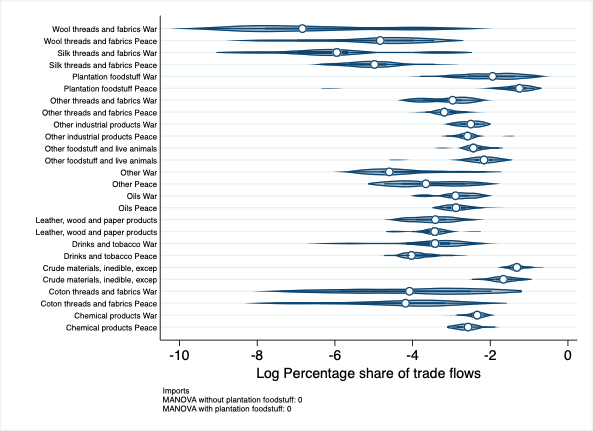
\includegraphics[scale=.4]{peace_war_nat_distr_Isitc}
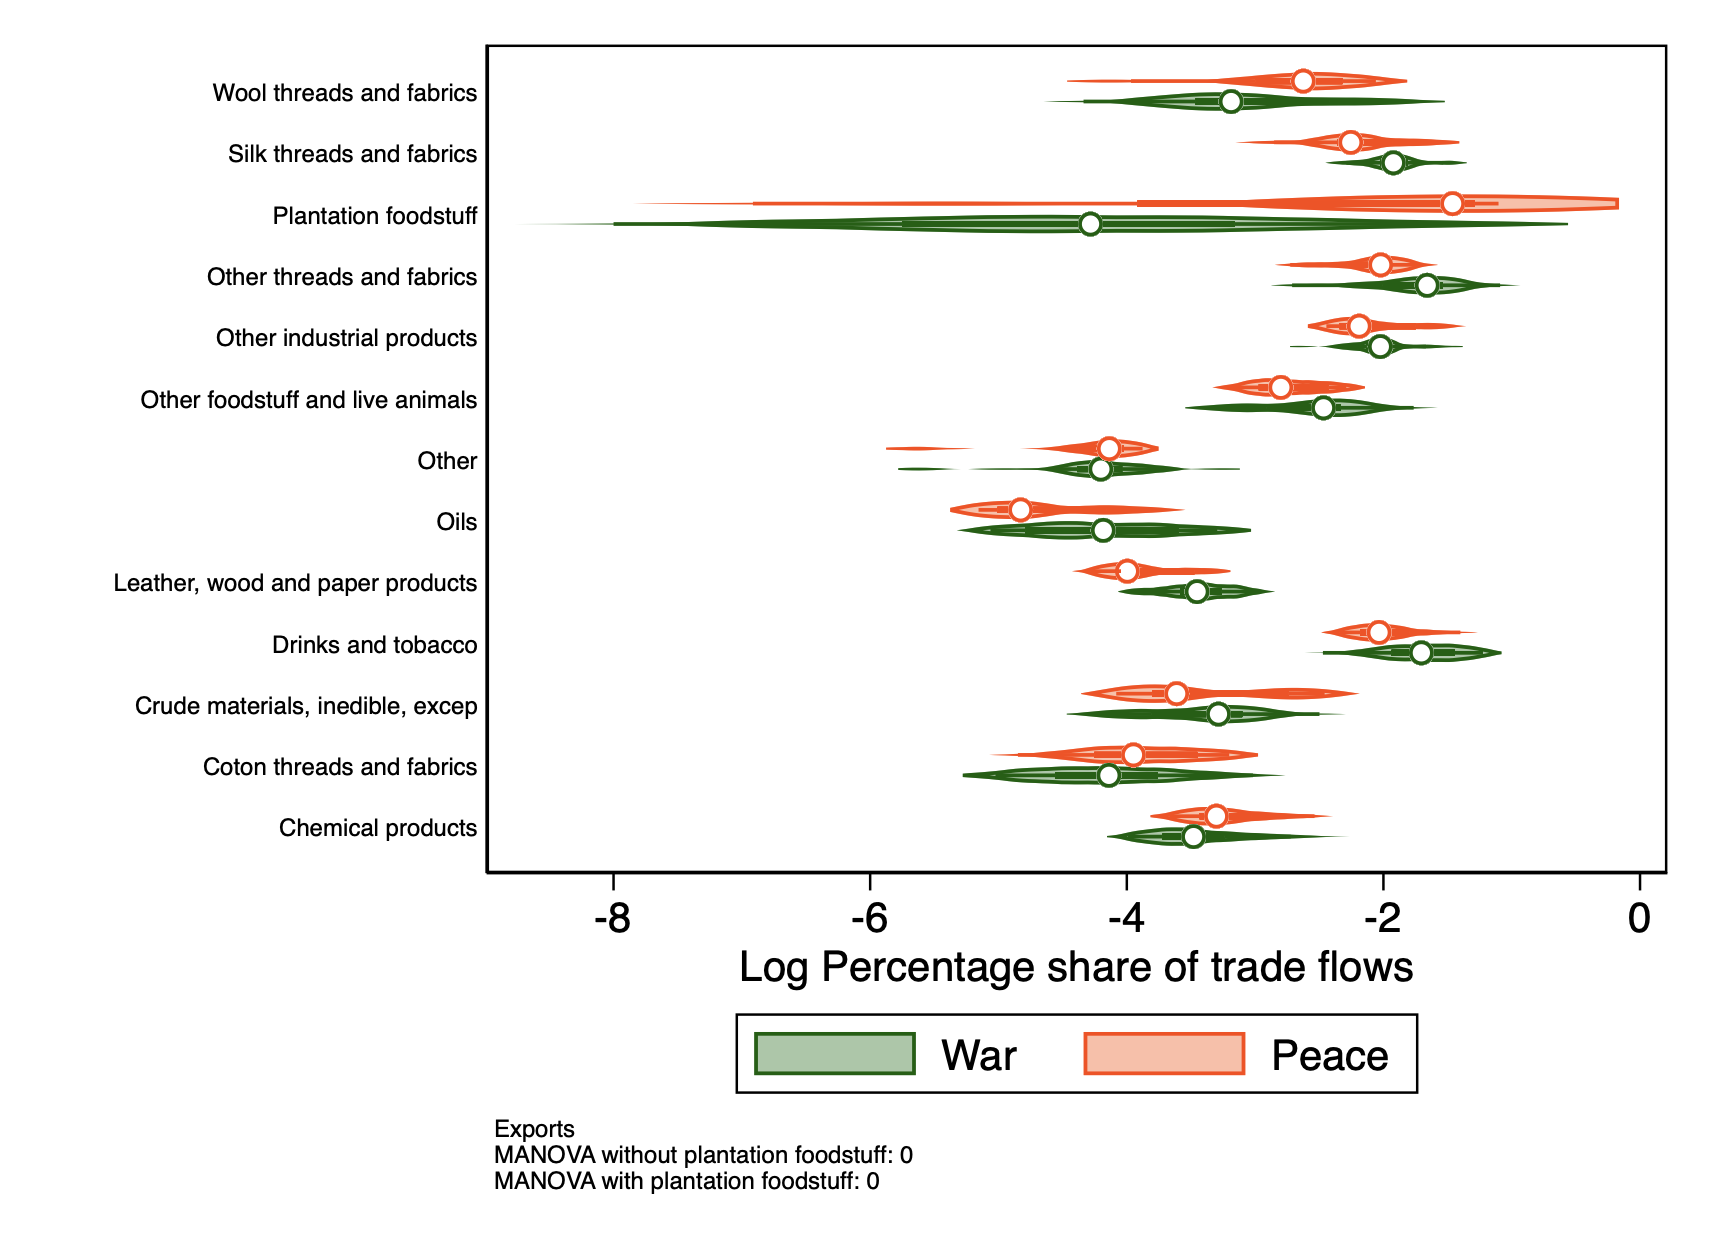
\includegraphics[scale=.4]{peace_war_nat_distr_Xsitc}
\end{figure}

\begin{figure}
\centering
\caption{American Independence War and Peace 1764-1777}
\label{peace1764_1777_indep_nat_distr_sitc}
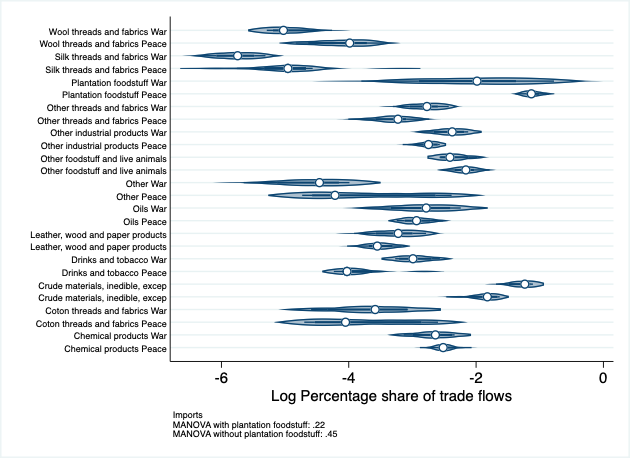
\includegraphics[scale=.4]{peace1764_1777_indep_nat_distr_Isitc}
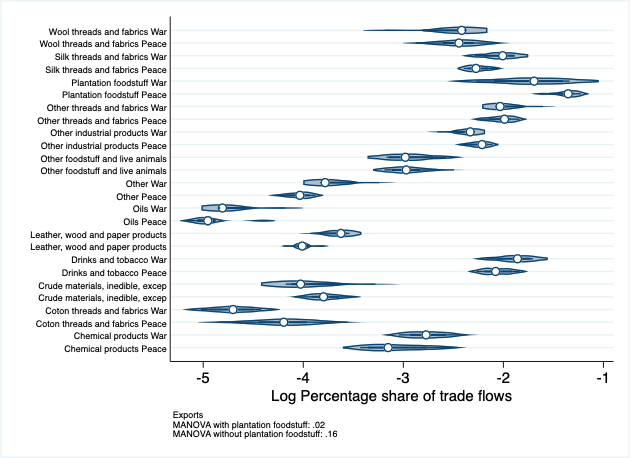
\includegraphics[scale=.4]{peace1764_1777_indep_nat_distr_Xsitc}
\end{figure}

\begin{figure}
\centering
\caption{Peace 1816-1840 and Continental Blockade}
\label{peace1816_1840_block_nat_distr_sitc}
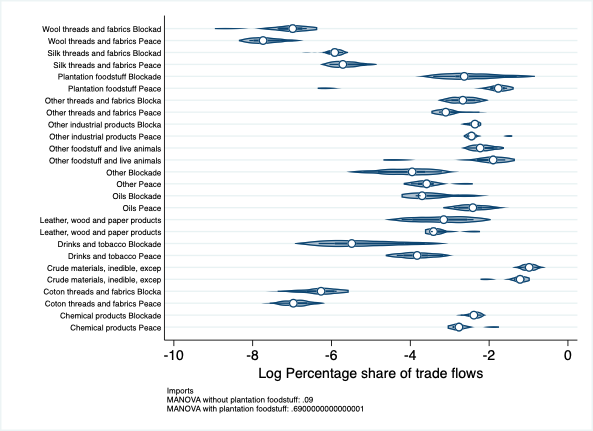
\includegraphics[scale=.4]{peace1816_1840_block_nat_distr_Isitc}
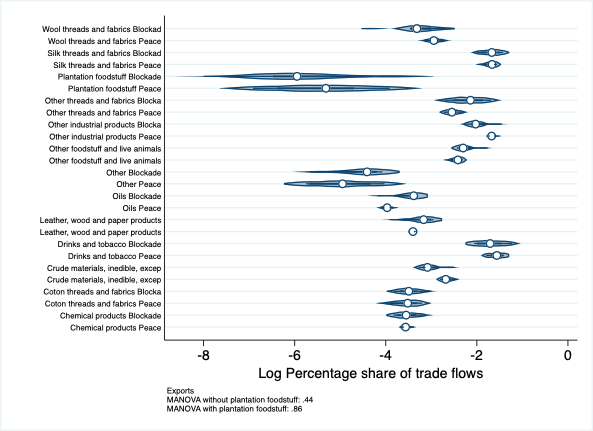
\includegraphics[scale=.4]{peace1816_1840_block_nat_distr_Xsitc}
\end{figure}

\begin{figure}
\centering
\caption{Revolutionary War and Continental Blockade}
\label{rev_block_nat_distr_sitc}
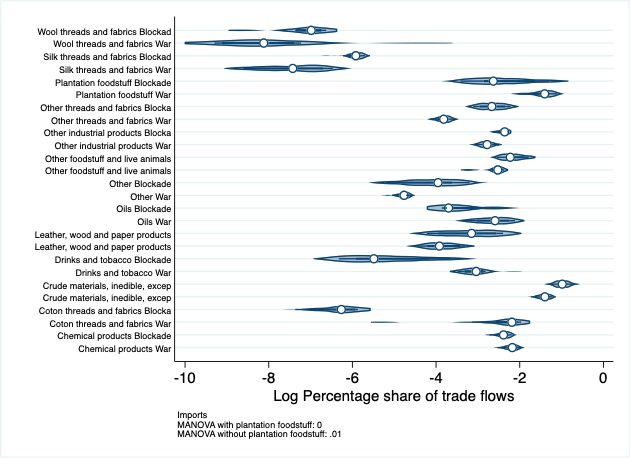
\includegraphics[scale=.4]{rev_block_nat_distr_Isitc}
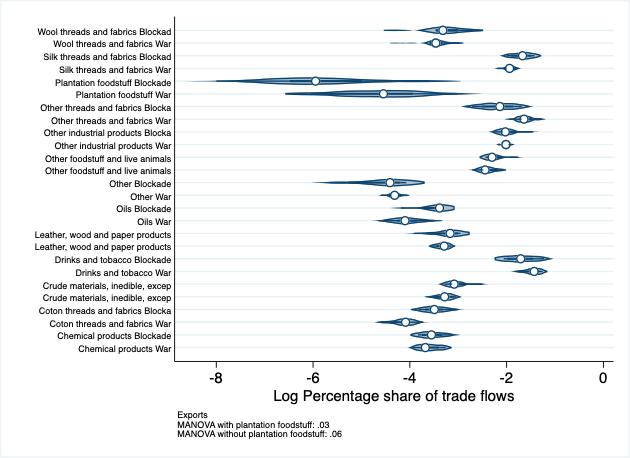
\includegraphics[scale=.4]{rev_block_nat_distr_Xsitc}
\end{figure}

\begin{figure}
\centering
\caption{Seven Years War and Peace 1816-1821}
\label{seven_peace1764_1777_nat_distr_sitc}
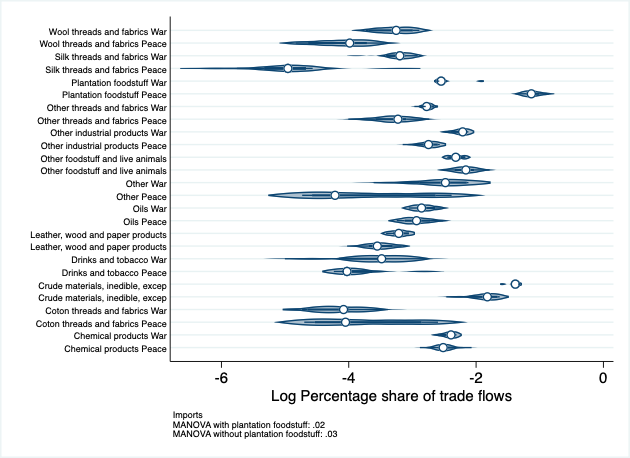
\includegraphics[scale=.4]{seven_peace1764_1777_nat_distr_Isitc}
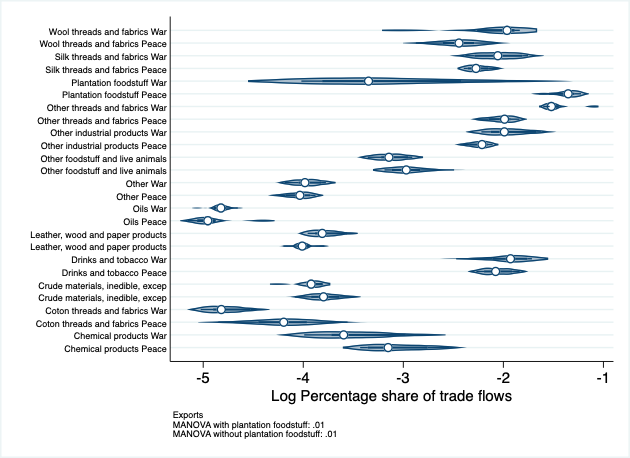
\includegraphics[scale=.4]{seven_peace1764_1777_nat_distr_Xsitc}
\end{figure}

\begin{figure}
\centering
\caption{Peace 1749-1755 and Peace 1764-1777}
\label{seven_peace1764_1777_nat_distr_sitc}
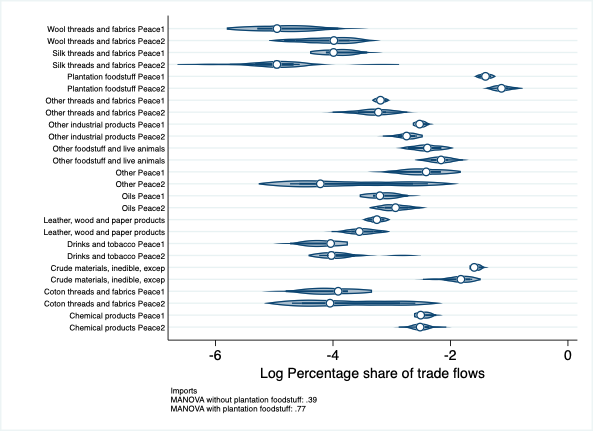
\includegraphics[scale=.4]{peace1749_1755_peace1764_1777_nat_distr_Isitc}
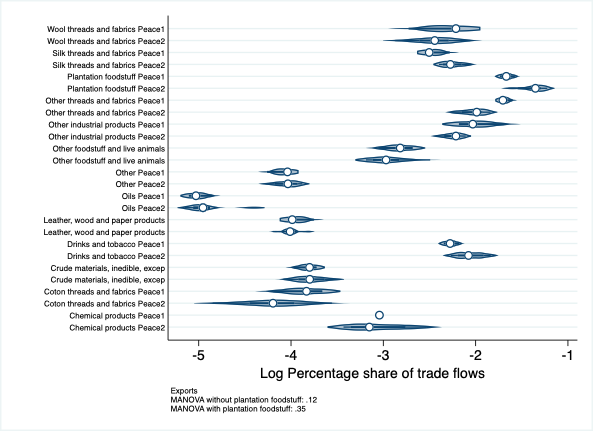
\includegraphics[scale=.4]{peace1749_1755_peace1764_1777_nat_distr_Xsitc}
\end{figure}

\begin{figure}
\centering
\caption{Peace 1764-1777 and Peace 1784-1792}
\label{seven_peace1764_1777_nat_distr_sitc}
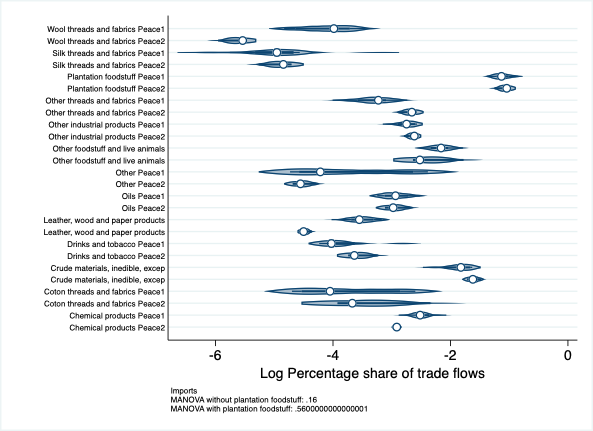
\includegraphics[scale=.4]{peace1764_1777_peace1784_1792_nat_distr_Isitc}
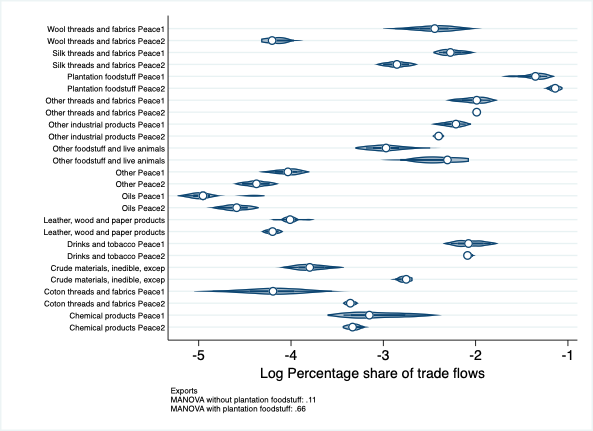
\includegraphics[scale=.4]{peace1764_1777_peace1784_1792_nat_distr_Xsitc}
\end{figure}

\begin{figure}
\caption{All War and Peace period}
\label{peace_war_nat_distr_pays7}
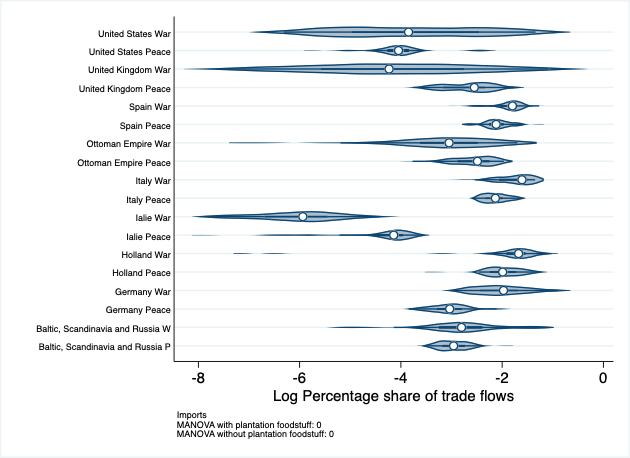
\includegraphics[scale=.4]{peace_war_nat_distr_Ipays7}
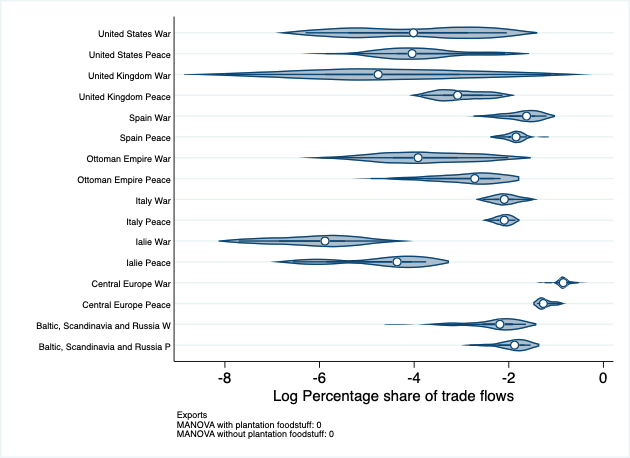
\includegraphics[scale=.4]{peace_war_nat_distr_Xpays7}
\end{figure}

\begin{figure}
\centering
\caption{American Independence War and Peace 1764-1777}
\label{peace1764_1777_indep_nat_distr_pays7}
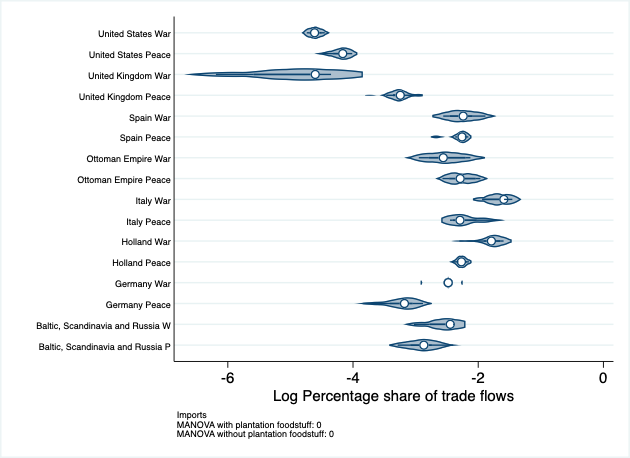
\includegraphics[scale=.4]{peace1764_1777_indep_nat_distr_Ipays7}
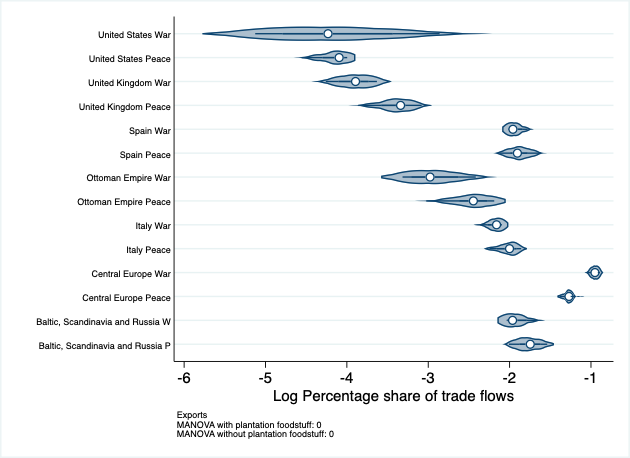
\includegraphics[scale=.4]{peace1764_1777_indep_nat_distr_Xpays7}
\end{figure}

\begin{figure}
\centering
\caption{Peace 1816-1840 and Continental Blockade}
\label{peace1816_1840_block_nat_distr_pays7}
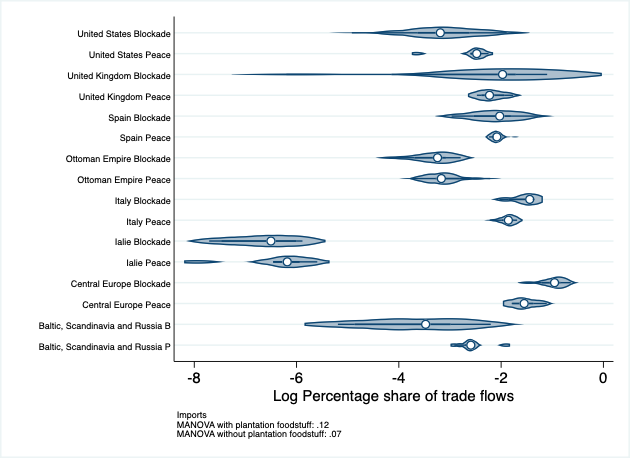
\includegraphics[scale=.4]{peace1816_1840_block_nat_distr_Ipays7}
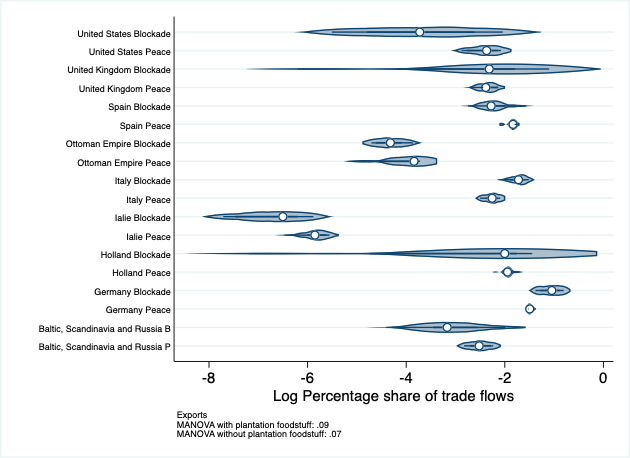
\includegraphics[scale=.4]{peace1816_1840_block_nat_distr_Xpays7}
\end{figure}

\begin{figure}
\centering
\caption{Revolutionary War and Continental Blockade}
\label{rev_block_nat_distr_pays7}
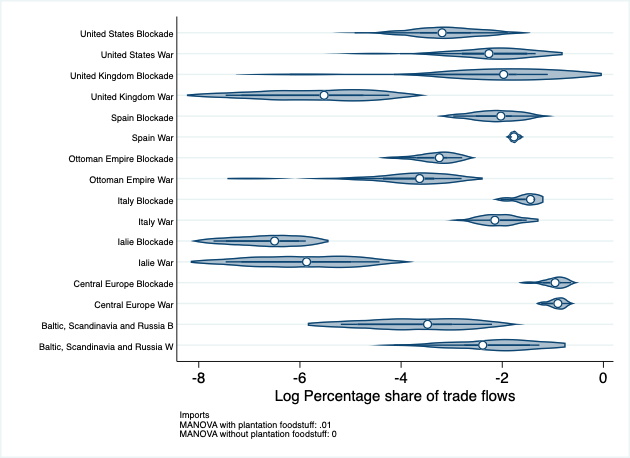
\includegraphics[scale=.4]{rev_block_nat_distr_Ipays7}
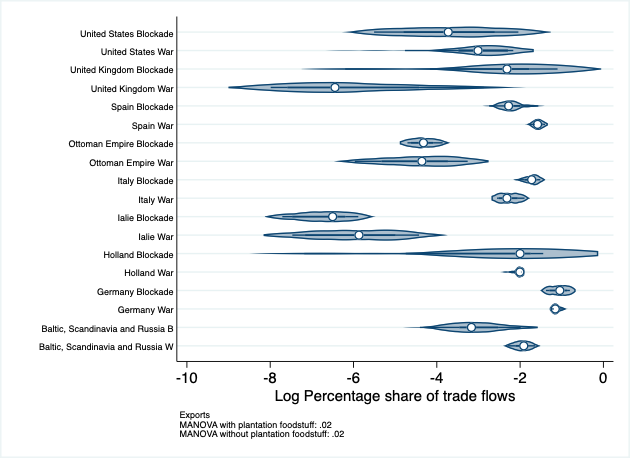
\includegraphics[scale=.4]{rev_block_nat_distr_Xpays7}
\end{figure}

\begin{figure}
\centering
\caption{Seven Years War and Peace 1816-1821}
\label{seven_peace1764_1777_nat_distr_pays7}
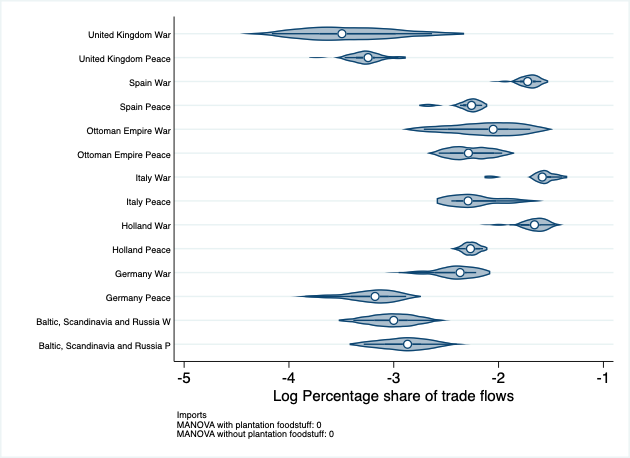
\includegraphics[scale=.4]{seven_peace1764_1777_nat_distr_Ipays7}
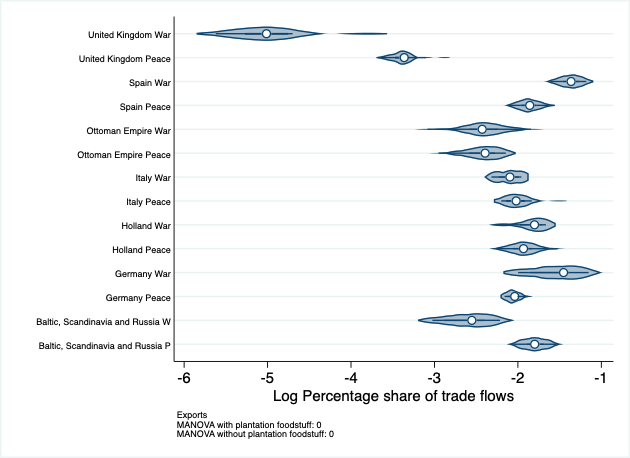
\includegraphics[scale=.4]{seven_peace1764_1777_nat_distr_Xpays7}
\end{figure}

\begin{figure}
\centering
\caption{Peace 1749-1755 and Peace 1764-1777}
\label{seven_peace1764_1777_nat_distr_pays7}
\includegraphics[scale=.4]{peace1749_1755_peace1764_1777_nat_distr_Ipays7}
\includegraphics[scale=.4]{peace1749_1755_peace1764_1777_nat_distr_Xpays7}
\end{figure}

\begin{figure}
\centering
\caption{Peace 1764-1777 and Peace 1784-1792}
\label{seven_peace1764_1777_nat_distr_pays7}
\includegraphics[scale=.4]{peace1764_1777_peace1784_1792_nat_distr_Ipays7}
\includegraphics[scale=.4]{peace1764_1777_peace1784_1792_nat_distr_Xpays7}
\end{figure}

\begin{figure}
\centering
\caption{Peace 1784-1792 and Peace 1816-1821}
\label{peace1784_1792_peace1816_1821_nat_distr_pays7}
\includegraphics[scale=.4]{peace1784_1792_peace1816_1840_nat_distr_Ipays7}
\includegraphics[scale=.4]{peace1784_1792_peace1816_1840_nat_distr_Xpays7}
\end{figure}

\begin{figure}
\caption{All War and Peace period}
\label{peace_war_nat_distr_aggr}
\includegraphics[scale=.4]{peace_war_nat_distr_Iaggr}
\includegraphics[scale=.4]{peace_war_nat_distr_Xaggr}
\end{figure}

\begin{figure}
\centering
\caption{American Independence War and Peace 1764-1777}
\label{peace1764_1777_indep_nat_distr_aggr}
\includegraphics[scale=.4]{peace1764_1777_indep_nat_distr_Iaggr}
\includegraphics[scale=.4]{peace1764_1777_indep_nat_distr_Xaggr}
\end{figure}

\begin{figure}
\centering
\caption{Peace 1816-1840 and Continental Blockade}
\label{peace1816_1840_block_nat_distr_aggr}
\includegraphics[scale=.4]{peace1816_1840_block_nat_distr_Iaggr}
\includegraphics[scale=.4]{peace1816_1840_block_nat_distr_Xaggr}
\end{figure}

\begin{figure}
\centering
\caption{Revolutionary War and Continental Blockade}
\label{rev_block_nat_distr_aggr}
\includegraphics[scale=.4]{rev_block_nat_distr_Iaggr}
\includegraphics[scale=.4]{rev_block_nat_distr_Xaggr}
\end{figure}

\begin{figure}
\centering
\caption{Seven Years War and Peace 1816-1821}
\label{seven_peace1764_1777_nat_distr_aggr}
\includegraphics[scale=.4]{seven_peace1764_1777_nat_distr_Iaggr}
\includegraphics[scale=.4]{seven_peace1764_1777_nat_distr_Xaggr}
\end{figure}

\begin{figure}
\centering
\caption{Peace 1749-1755 and Peace 1764-1777}
\label{seven_peace1764_1777_nat_distr_aggr}
\includegraphics[scale=.4]{peace1749_1755_peace1764_1777_nat_distr_Iaggr}
\includegraphics[scale=.4]{peace1749_1755_peace1764_1777_nat_distr_Xaggr}
\end{figure}

\begin{figure}
\centering
\caption{Peace 1764-1777 and Peace 1784-1792}
\label{seven_peace1764_1777_nat_distr_aggr}
\includegraphics[scale=.4]{peace1764_1777_peace1784_1792_nat_distr_Iaggr}
\includegraphics[scale=.4]{peace1764_1777_peace1784_1792_nat_distr_Xaggr}
\end{figure}

\begin{figure}
\centering
\caption{Peace 1784-1792 and Peace 1816-1821}
\label{peace1784_1792_peace1816_1840_nat_distr_Iaggr}
\includegraphics[scale=.4]{peace1784_1792_peace1816_1840_nat_distr_Iaggr}
\includegraphics[scale=.4]{peace1784_1792_peace1816_1840_nat_distr_Xaggr}
\end{figure}

\section{Conclusion} \label{conclusion}
In this paper we have analysed the effects of different conflicts on French trade in the eighteenth century.
We have first created a loss measure by comparing the amount of trade that would have taken place in the absence of conflicts with the observed trade.
We have done so both by using all the preceding peace periods to compute expected trade and just the period immediately before the conflict.
From this computation we have observed mainly two things; first that the main losses were during the Seven Years War and the Revolutionary Wars-Continental Blockade, second that only as a consequence of these two conflicts there were long lasting effects.
This leads us to think that there must have been a common factor that made these two wars so disruptive.
We analyse several cases.
Naval supremacy is a possible explanation and for this reason we construct a measure to account for it.
We take the ratio first of France and Great Britain's number of warships, then that of France and Great Britain including their allies, and finally France with neutral countries and Great Britain including their allies.
Contrary to our expectations, we find rather a positive relation, meaning that an increase in the number of warship was linked to a bigger loss in trade.
This can possibly be explained by the fact that countries were investing in their navies in the attempt to protect their trade or to fight wars.
However, this does not seem to explain the loss in trade per-se. Another option was the loss of colonies.
Especially towards the end of the century, France lost some of its richest colonies, which had a consequence on their imports.
We have created a measure to account for the colonies loss, weighted for the share of trade those colonies accounted for.
We find in this case little more correlation with the loss function, however this does still not entirely explain the losses of the Seven Years War, nor the fluctuations in this measure seem to be related to the loss in the Blockade period.
Finally, we have investigated the policy towards neutral countries, which had been changing throughout the century.
We find that, whenever the policy with respect to trade with neutral countries were looser, war losses were limited and commerce could recover its pre-war level very quickly, even outperform it.
On the other hand, when the British started blockading neutral countries as well, French trade experienced a massive drop and a long convalescence. \\
We conclude that, even if all these factors probably were contributing to the loss in trade during conflicts, the turning point was strictly related to policy towards neutral countries.
British could efficiently curtail French trade only by blockading neutral countries.


\pagebreak

\renewcommand{\baselinestretch}{1.0}\normalsize

\bibliographystyle{apalike}
\bibliography{How_to_wage_a_trade_war}

%plainnat


\end{document}

